\documentclass[review]{elsarticle}
\usepackage[bottom=22.1mm, top=16mm, left=25mm, right=25mm]{geometry}
\usepackage{float}
\usepackage{amssymb, amsmath}
\usepackage{import}
\usepackage{xcolor}
\usepackage{graphicx}
\usepackage{siunitx}
\usepackage{lineno}
\usepackage{tabularx}                   % For adjustable-width tables
\usepackage{booktabs}                   % For professional-looking tables
\usepackage{subcaption}                 % Allows to add subcations in subplots
\usepackage{setspace}                   % Package to be used for setting custom line spacing.
\usepackage{pdfpages}                   % To attach PDF documents to the output.
\usepackage{fancyhdr}                   % For headers and footers.
\usepackage{minted}                     % Package for listing codes.
\usepackage[bottom]{footmisc}           % Aligns footnote to the bottom of the page.
\usepackage[ruled, vlined]{algorithm2e} % Package for write algorithms
\usepackage{fontawesome5}               % Addition of icons to the document.
\usepackage[hidelinks]{hyperref}               % Duckies
\usepackage{comment}                    % Used for adding comments to the document
\usepackage{svg}                        % To include svg format files
\usepackage[version=4,arrows=pgf-filled,textfontname=sffamily,
mathfontname=mathsf]{mhchem}            % Chemistry package

% Document settings
\modulolinenumbers[10]
\SetAlFnt{\footnotesize}
\bibliographystyle{elsarticle-num}

\journal{Dr. Jerin John for MECH 6191 W2025.}

%%%%%%%%%%%%%%%%%%%%%%%


\begin{document}
\setstretch{1.15}
\begin{frontmatter}


\title{Rich-Quench-Lean Combustion using Ammonia \tnoteref{mytitlenote}}
\tnotetext[mytitlenote]{Fully documented code is available on \href{https://github.com/paramvirlobana/Combustion-W2025}{\faGithub\ github/Combustion-W2025}. Short developer guide presented in the Appendix.}

%% Group authors per affiliation:
\author[add1]{Paramvir }

\address[add1]{Department of Mechanical, Industrial and Aerospace Engineering, \\ Concordia University \\ Montreal, QC, Canada}

\begin{abstract}
In this project, the use of rich-burn, quick-mix, lean-burn (RQL) combustion to reduce \ce{NOx} emissions in amonia-fueled systems. Generally, ammonia is a promising clean fuel. However, it poses challenges due to high \ce{NOx} formation in lean premixed combustion. To address this issue, RQL provides a solution by initiating combustion in a fuel-rich environment that suppresses \ce{NOx} formation with a rapid air mixing and a final combustion in a lean zone. This combustion process is modeled in Cantera by coupling 3 reactors in series: a combustor rich burn zone, a mixer with secondary air addition, a combustor lean burn zone. In addition to this, numerical simulation is done using Ansys that uses a simplified RQL combustion geometry with defined zones for fuel injection, air mixing, and lean burn. Performance is then evaluated on the basis of emissions. This study shows the potential of RQL combustion that reduces \ce{NOx} emissions.
\end{abstract}


\begin{keyword}
RQL \sep Ammonia \sep Combustion \sep Cantera \sep ANSYS
\end{keyword}

\end{frontmatter}
\linenumbers % -> This is for the line numbers on the left hand side of the page.

%%%%%%%%%%%%%%%%%%%%%%%%%%%%%%%%%%%%%%%%%%%%%%%%%%%%%%%%%%%%%%%%%%%%%%%%%%%%%%%%%%%%%%%%%%%%%%%%%
%                                   END OF THE FRONT MATTER
%%%%%%%%%%%%%%%%%%%%%%%%%%%%%%%%%%%%%%%%%%%%%%%%%%%%%%%%%%%%%%%%%%%%%%%%%%%%%%%%%%%%%%%%%%%%%%%%%

\section{Background}
This section talks about the process of the RQL reaction mechanism.





Boundary conditions:




T in fuel   = 500 K

T in air    = 800 K  

P in fuel   = 15 bar

P in air    = 12 bar  




%\begin{figure}[H]
%    \centering
%    \includesvg[width=0.7\linewidth]{figs/rql_process_diagram.svg}
%    \caption{Caption}
%    \label{fig:enter-label}
%\end{figure}


Writing the balanced chemical equation

\begin{equation}
    \ce{4NH3 + 3(O2 + 3.76 N2) -> 2N2 + 6H2O + 11.28N2}\label{eq:balanced_reaction}
\end{equation}

In \autoref{eq:balanced_reaction}, the oxidizer nitrogen is kept separate from the inert air nitrogen to keep track.


\section{Combustor Design}
The three dimensional geometry of the non-premixed swirl combustor chamber an it's central cross-sectional dimensions are presented in \autoref{fig:model_rql}. The combustion chamber constitutes 
of a rich burn region with a fuel inlet at the centre. The ring around the fuel inlet is the primary air inlet. There are 16 air holes downstream of the combustion chamber 
to deliver the secondary air for the lean combustion zone. The combustion chamber has been designed in such a way that for specific mass flows, rich combustion can take place
in the rich region and after adding the secondary air, the NOx can be reduced using lean combustion.

\subsection{Boundary Conditions}

The equivalence ratio of the primary combustion zone has been set to 1.24 and the global equivalence ratio has been set to 0.42. Both of these quantities are design choices
and have helped derive the combustor geometry. The fuel and air temperature used for this study have been adopted from reference \cite{wang2023non}. The combustor specifications
and the boundary conditions are summarized in \autoref{tab:air_fuel_properties}. The fuel pressure has been set higher that the air pressure to avoid back flow.

\begin{table}[H]
    \centering
    \caption{Boundary conditions.}\label{tab:air_fuel_properties}
    \begin{tabular}{lcc}
    \toprule
    & Temperature [K] & Pressure [MPa] \\
    \midrule
    Air  & 800  & 12 \\
    Fuel & 325  & 15 \\
    \bottomrule
    \end{tabular}
\end{table}

The following subsections discuss the conditions at the two different zones of combustion in detail. An important parameter to note here is the momentum flux ratio ($J$).
The momentum flux ratio is a critical parameter in combustion systems, defined as the ratio of momentum flux of the fuel to that of the air. It influences flame stability, mixing, and combustion efficiency. Mathematically, it can be defined as:

\begin{equation}
    J = \frac{\rho_{\text{jet}} u_{\text{jet}}^2}{\rho_{\infty} u_{\infty}^2}
\end{equation}

\subsection{Rich Burn Zone}

As mentioned before, the equivalence ratio for the rich burn zone has been set to $\phi_{\text{rich}} = 1.24$ as a design choice.
Literature \cite{Talpallikar1992} suggests that an acceptable $J$ for a inlet swirl type combustor should be between 2-3, which has been set as a constraint for this design.


Writing the balanced chemical equation:


\begin{equation}
    \ce{4NH3 + 3(O2 + 3.76 N2) -> 2N2 + 6H2O + 11.28N2}\label{eq:balanced_reaction}
\end{equation}

In \autoref{eq:balanced_reaction}, the oxidizer nitrogen is kept separate from the inert air nitrogen to keep track. The air-fuel ratio can be expressed as:

\begin{equation}
    \left( \frac{A}{F} \right) = \frac{N_{\text{air}}}{N_{\text{fuel}}} \times \frac{MW_{\text{air}}}{MW_{\text{fuel}}}
\end{equation}

From the balanced reaction in \autoref{eq:balanced_reaction}:

\begin{equation}
    \left( \frac{A}{F} \right)_{\text{stoic}} = 4.76 \times 0.75 \times \frac{28.85 \; \text{g/mol}}{17.034 \; \text{g/mol}} = 6.05
\end{equation}


Therefore, using the above relation, the air-fuel ratio for a rich combustion configuration can be obtained:

\begin{equation}
    \phi = \frac{(A/F)_{\text{stoic}}}{(A/F)_{\text{required}}}
\end{equation}

The required air-fuel ratio for $\phi = 1.24$ is computed as follows:

\begin{equation}
    (A/F)_{\text{required}} = \frac{(A/F)_{\text{stoic}}}{\phi} = \frac{6.05}{1.25} = 4.854
\end{equation}

Therefore, $\phi$ and $(A/F)$ have been set for the rich combustion have been set so far. The next step is to obtain the inlet mass flow rates for the 
fuel and the air for this design. It is known that $\dot{m} = \rho V A$. Area is known from the geometry. $\rho$ for air and fuel can be obtained from the respective fluid properties. Hence,
the mass flow for both the air and fuel can be obtained using the respective inlet velocities. A range for both $U_{\text{air}}$ and $U_{\text{fuel}}$ as well as $J$ have been used:

\begin{table}[H]
\centering
    \begin{tabular}{ll}
         $J$              &  2 - 3 \\
         $U_{\text{air}}$ &  40 m/s to 90 m/s \\
        $U_{\text{fuel}}$ &  60 m/s to 110 m/s \\
    \end{tabular}
\end{table}

After iterating over the above ranges, the results are filtered based on the required $\phi$ and $J$. The program used has been presented in Appendix \ref{subsection:primary_calcs}.
The chosen operating conditions for this region are presented in \autoref{tab:air_fuel_properties}. The program helps obtain the inlet mass flow rates for the fuel and the oxidizer. The results used in the analysis presented in this report are below:

\begin{table}[H]
    \centering
    \begin{tabular}{ll}
         Primary inlet mass flow rate &  0.035631 kg/s\\
         Fuel mass flow rate &  0.007339 kg/s
    \end{tabular}
\end{table}


These conditions have been used to set the boundary conditions for the numerical analysis which will be discussed in a later section.


\subsection{Lean Burn Zone}

Literature suggests that a momentum flux ratio of 40 in the mixing zone should induce enough turbulence in the zone to mix the secondary air with the downstream gases from the rich combustion zone. Therefore, the momentum flux ratio for this region has be set to 40 as a design choice \cite{Talpallikar1992, Lefebvre2010}. The objective is to calculate the secondary mass flow rate such the the global equivalence ratio becomes 0.42. This can be obtained by computing the global air-fuel ratio:

\begin{equation}
\begin{split}
        \left( A/F \right)_{\text{global}} & = \left( A/F \right)_{\text{stoic}} / \phi_{\text{global}} \\
        & = 4.854 / 0.42 \\
        & = 14.3993
\end{split}
\end{equation}

Then, the global mass flow rate can be calculated as:



\begin{equation}
\begin{split}
        \dot{m}_{\text{global}} & = \dot{m}_{F} \times  \left( A/F \right)_{\text{global}} \\
        & = 0.007339 \times 14.3993 \\
        & = 0.07004 \text{ kg/s}
\end{split}
\end{equation}

Therefore, a secondary mass flow rate of 0.07004 kg/s leads to a global equivalence ratio of 0.42 after the mixing/quench region.

\subsection{Swirler Design}

The primary zone airflow pattern is of prime importance to flame stability. For better mixing, one of the most effective ways of inducing flow recirculation in the primary zone is to fit a swirler in the dome around the fuel injector. This causes recirculation in the core region when the amount of rotation imparted to the flow is high. There are two main types of air swirles: axial and radial. In the presented design, an axial swirler is used. This is because it rotates the flow better in the tangential direction allowing it to evenly mix with the fuel jets. Typical ranges of values for the design of axial swirlers are \cite{dodds1990combustion, knight1953component}

\begin{table}[H]
    \centering
    \begin{tabular}{lll}
        \textbf{Parameter} & \textbf{Typical Value} & \textbf{Selected} \\
         Vane angle, $\theta$ &  30 - 60 deg & 45 deg \\
         Vane thickness, $t_{\nu}$ & 0.7 - 1.5 mm & 1.5 mm \\
         Number of Vanes, $n_{\nu}$ & 8 - 16 & 8
    \end{tabular}
\end{table}

\subsection{Final Design}

The general design of an RQL combustor has been adopted from existing designs being tested with ammonia as the fuel. One such design is presented in reference \cite{FATEHI20241} and shown in \autoref{fig:ref_rql_combustor}. It must be noted that the combustor used in this analysis is based on the reference combustor, however, many aspected have been changed. For example, the sleeve for the secondary air is replaced with a simple secondary air inlet zone and the while secondary air region has been removed for simplicity. 

\begin{figure}[H]
    \centering
    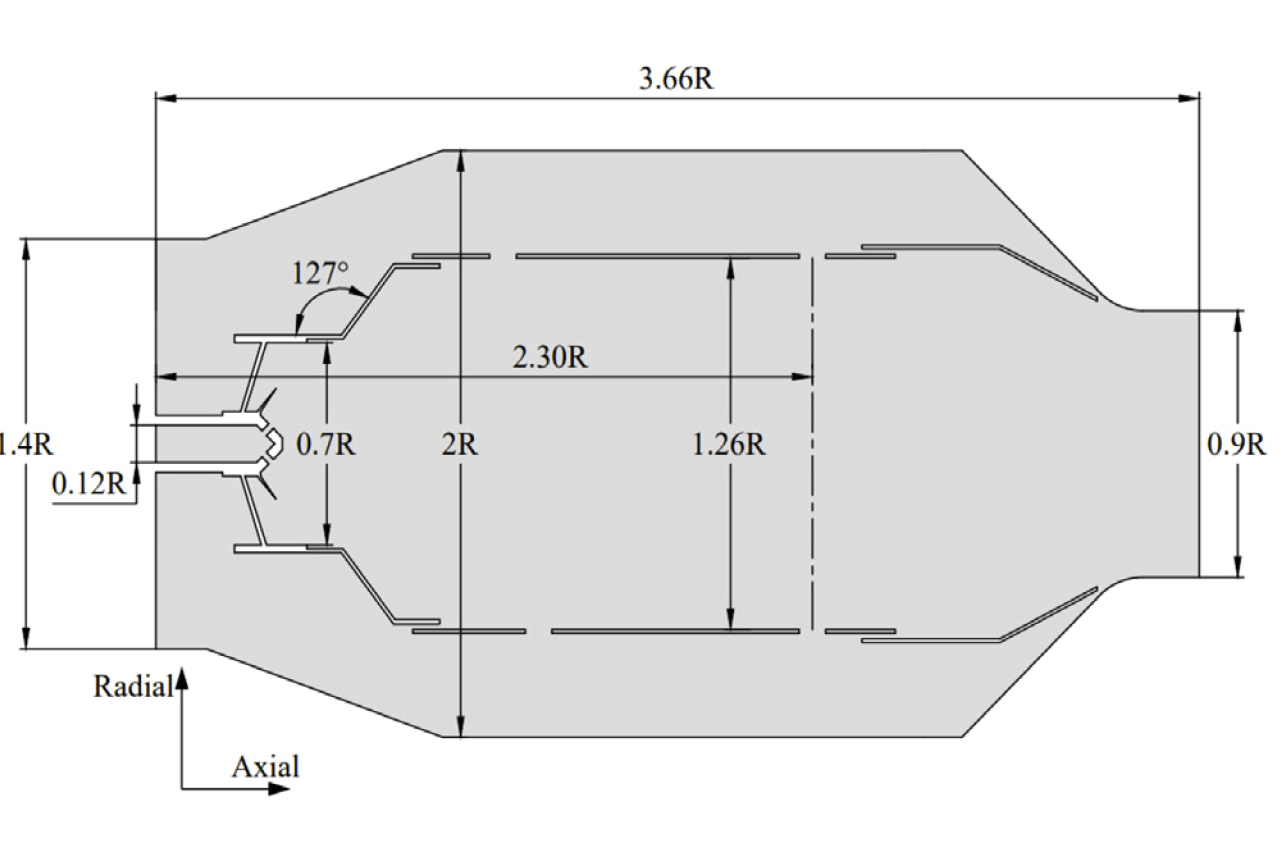
\includegraphics[width=0.5\linewidth]{figs/reference_rql_combustor.png}
    \caption{Central cross-sectional dimensions of the reference non-premixed swirl combustor \cite{samuelsen2006rich}.}\label{fig:ref_rql_combustor}
\end{figure}

Based on the analysis discussed in the previous sections, an RQL combustor is modelled and shown in \autoref{fig:model_rql}. The left figure shows the overall design and the right figure shows the details of the fuel injector. A detailed drawing with all the dimensions is presented in Appendix \ref{subsection:rql_dim_drawing}.

\begin{figure}[H]
    \centering
    \begin{subfigure}{0.49\linewidth}
      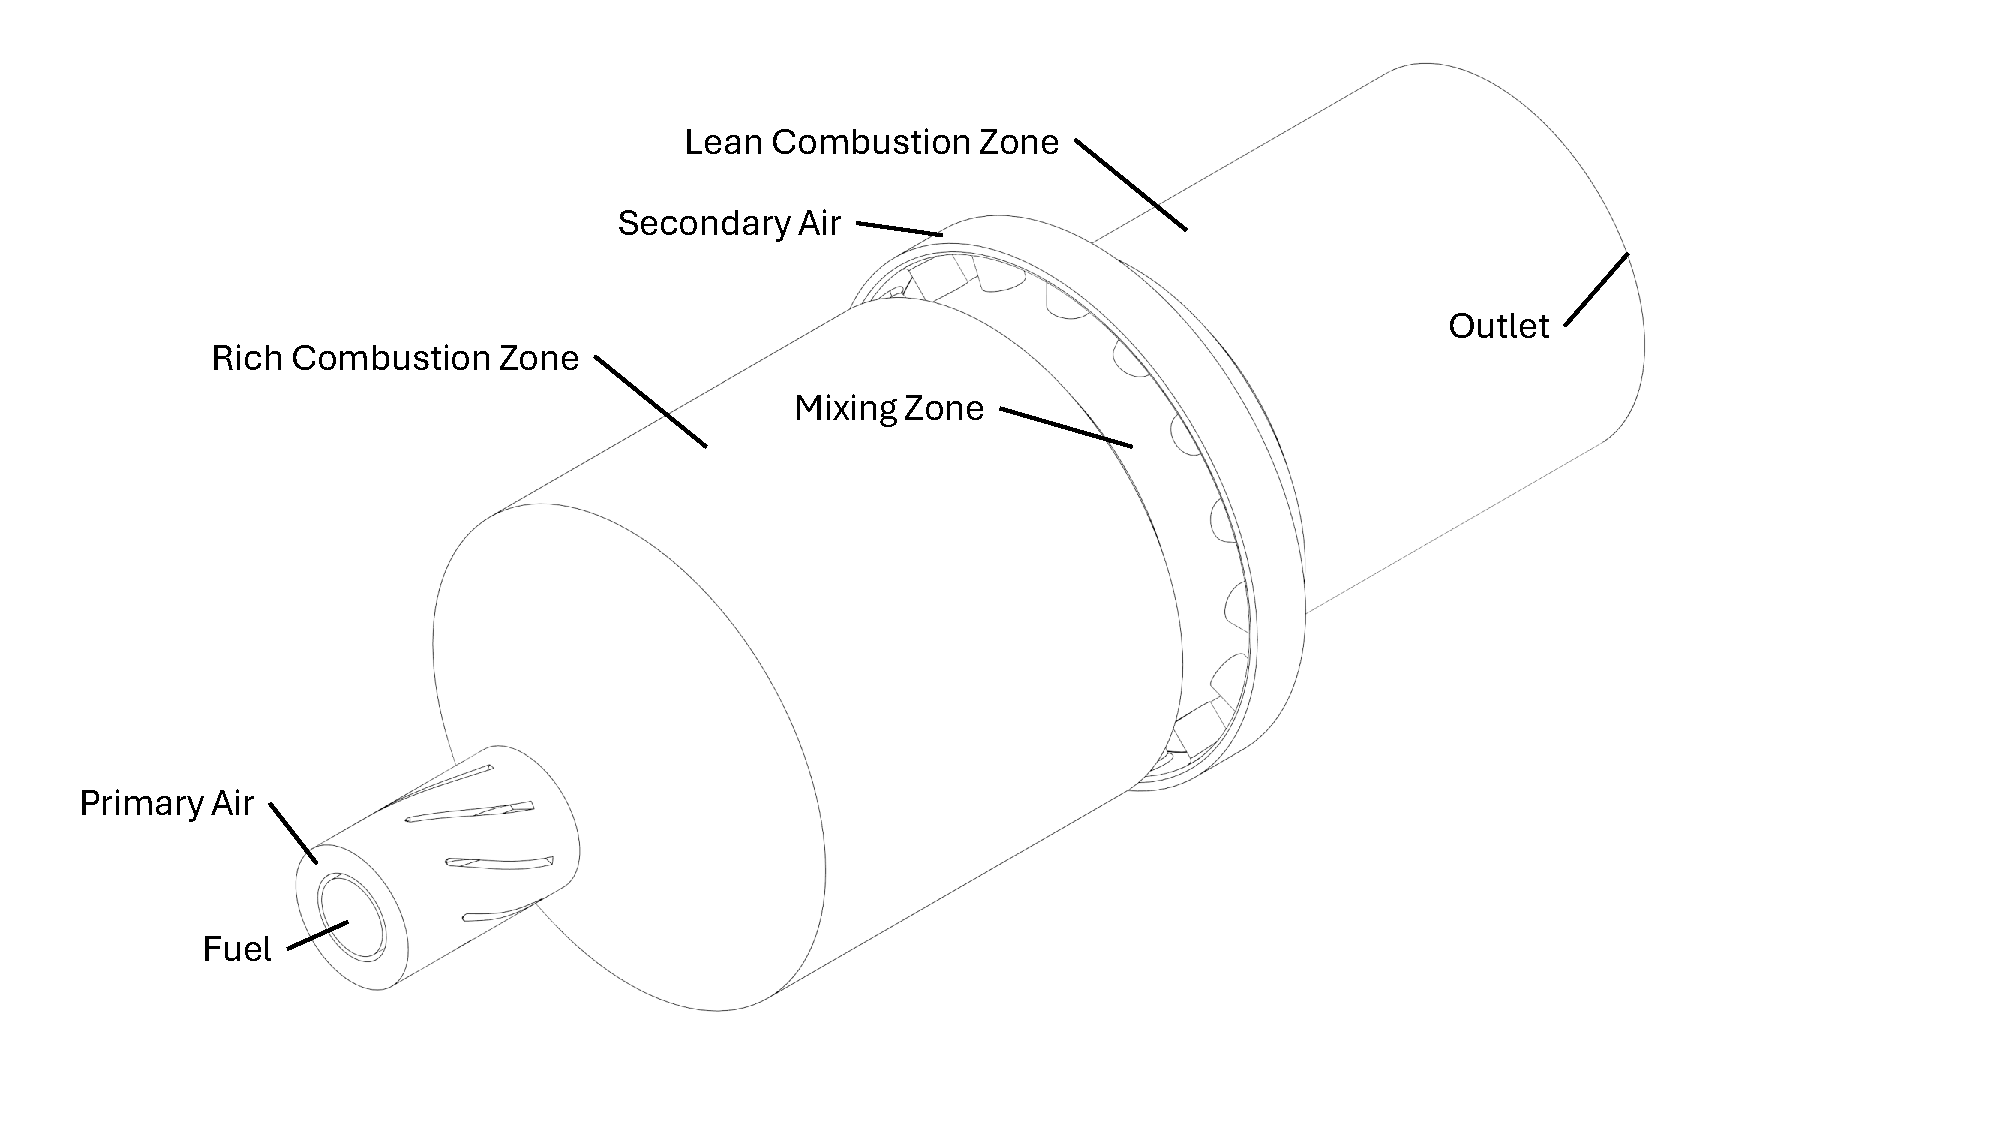
\includegraphics[width=\linewidth]{figs/overall_design.pdf}
    \end{subfigure}
    \hfill
    \begin{subfigure}{0.49\linewidth}
      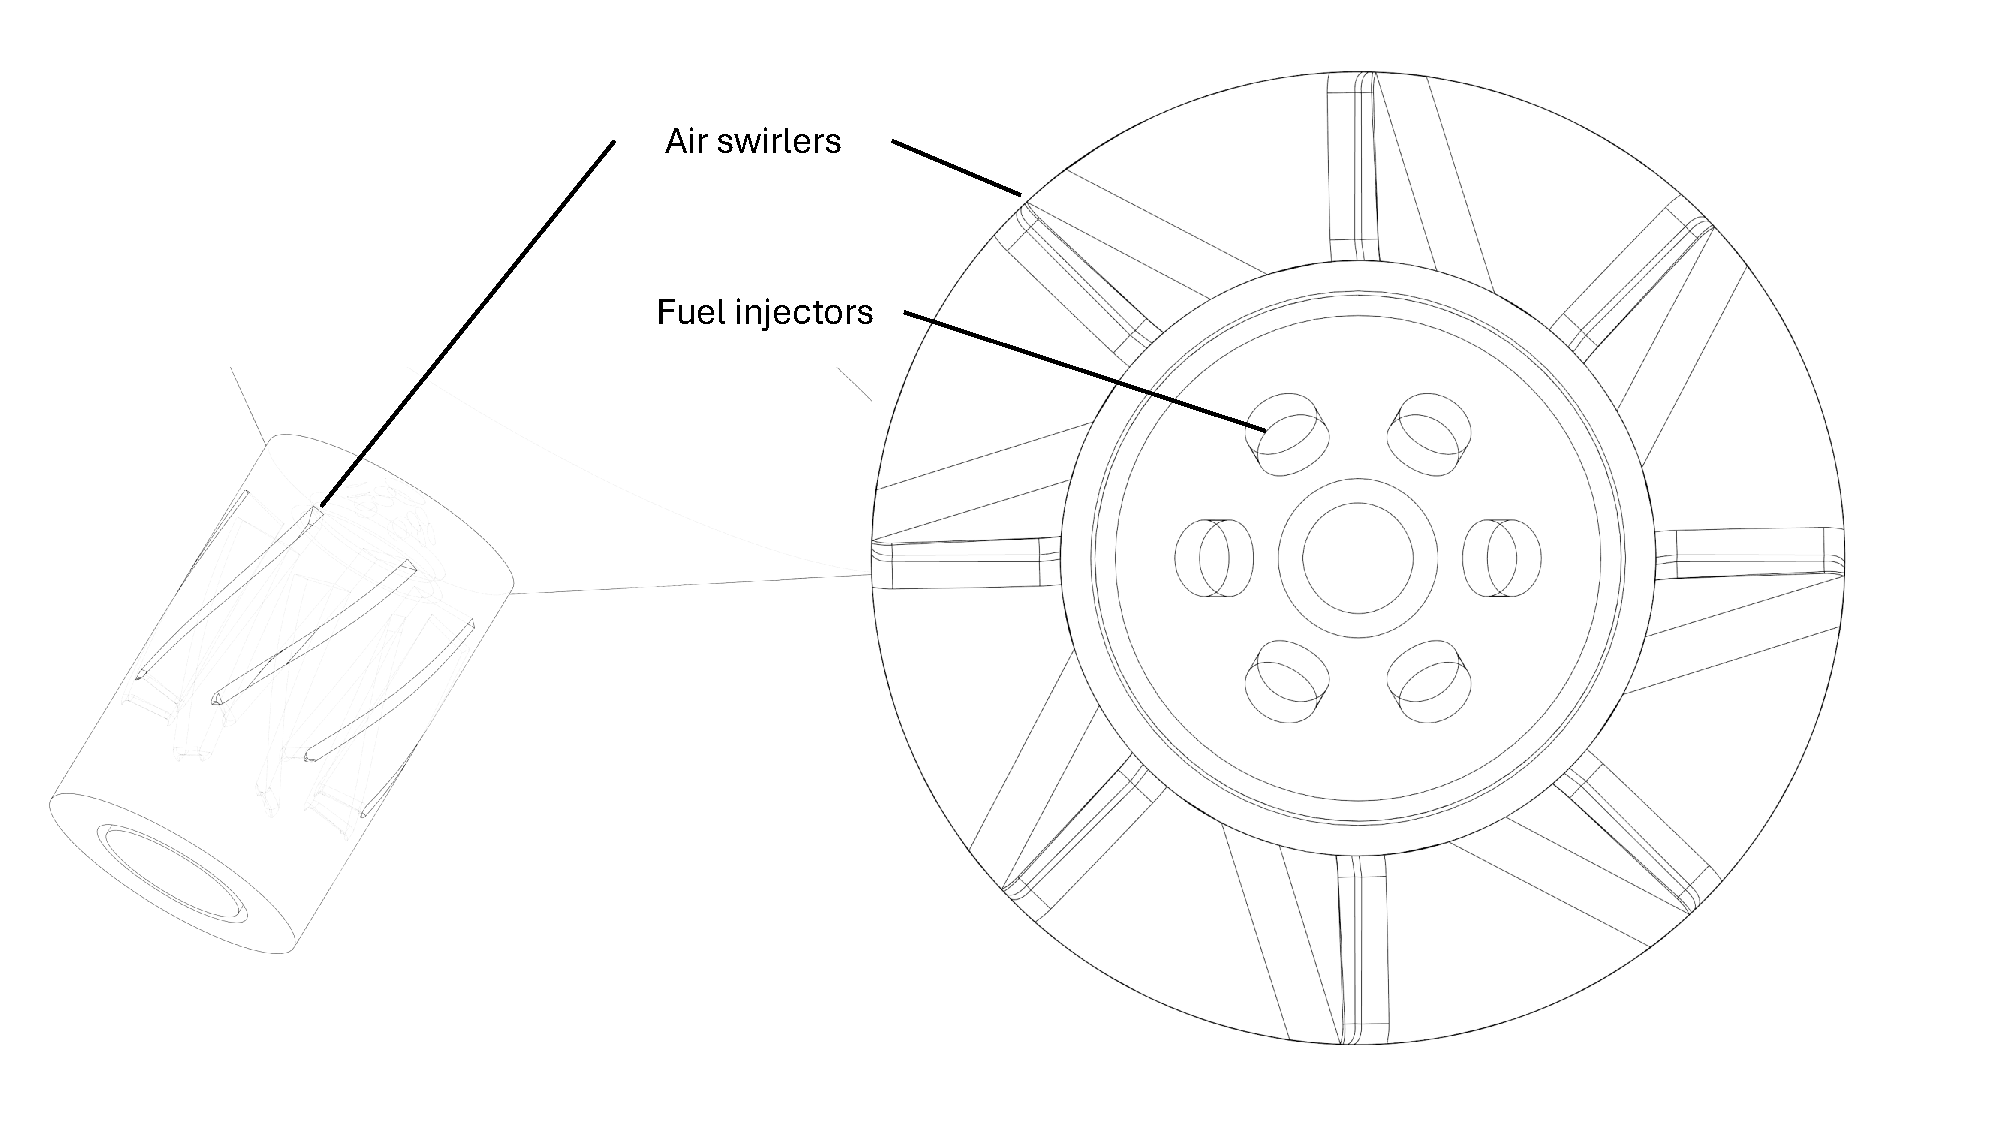
\includegraphics[width=\linewidth]{figs/injector.pdf}
    \end{subfigure}
\caption{Three dimensional model of the designed combustor.}\label{fig:model_rql}
\end{figure}





\section{Methodology}
The following subsections discuss the methodology used for setting up cantera and numerical simulations.


\subsection{Cantera} 

As discussed before, a generic RQL process has three main components: the rich combustion zone, the quick mix or quenching zone and the lean combustion zone. Therefore, to model such a system in cantera, three systems are needed as well. \autoref{fig:rql_process_diagram} presents a simple process diagram for such a model.

\begin{figure}[H]
    \centering
    \includesvg[width=0.7\linewidth]{figs/rql_process_diagram.svg}
    \caption{RQL combustor modelling process diagram.}\label{fig:rql_process_diagram}
\end{figure}

Since the scope of this project focuses in the combustion of ammonia, a mechanism is required to model it in cantera that is able to accurately capture the sub-mechanisms involved in the combustion of ammonia. Therefore, the SanDiego mechanism with a nitrogen sub-mechanism is used. The mechanism has to be manually generated from the chemkin files using cti2yaml utility provided by cantera. The publications on these mechanisms and the chemkin files are provided in reference \cite{SanDiegoMechanism}. The generated yaml file can be obtained from the Github repository of this project provided on the cover page.

\subsubsection{Rich Zone}

The first step is to initiate the states of the fuel and air in cantera. This is done by using the mechanism objects as seen below.

\begin{minted}[frame=lines,fontsize=\footnotesize,linenos, baselinestretch=1.0]{python}
    SanDiegoMech    =   os.path.join(MECHANISM_DIR, 'SanDiego.yaml')

    fuel        = ct.Solution(SanDiegoMech)
    fuel.TPX    = T_FUEL, P_FUEL, {'NH3': 1.0}

    air         = ct.Solution(SanDiegoMech)
    air.TPX     = T_AIR, P_AIR, {'O2': 1.0, 'N2': 3.76}
\end{minted}



Next step is to create a combustor for the rich zone. This is done using a one dimensional flame. Similar to the previous step, a new object called \textit{rich\_gas} is created to represent the gas exiting the rich combustion zone. Initial conditions are applied based on the mean values of the air and fuel temperature, pressure and mass fractions. A function called \textit{rich} is defined that solved the rich combustion using 1D flame. The FreeFlame object in cantera is used. Only the description for the function is presented below. For complete program, refer to the Appendix or the Github repository.

\begin{minted}[frame=lines,fontsize=\footnotesize,linenos, baselinestretch=1.0]{python}
    # Create the rich burn gas
    rich_gas = ct.Solution(SanDiegoMech)    
    rich_gas.TPY = rich_gas_thermo.thermo.T, rich_gas_thermo.thermo.P, rich_gas_thermo.thermo.Y
    rich_flame, rich_out, rich_outlet_state = rt.rich(eqr=1.24, mixture=rich_gas)

    # Function for the rich zone.
    def rich(
        eqr: float, mixture:ct.composite.Solution
    ) -> tuple:
        """
        Function for calculating the reaction characteristics in the rich burn zone.
       
        Inputs:
        ------
        - eqr_rich: equivalence ratio for the rich zone
        - mixture: init mixture gas
       
        Returns:
        -------
        - flame: solved FreeFlame object
        - gas_mix: cantera Solution object with the mixed state
        - outlet_state: string of species mass fractions at the outlet
        """
\end{minted}

\subsubsection{Quick Mix/Quench Zone}


 
After this zone, the hot gases need to be mixed with secondary zone. This is done by using the mixer class in cantera. See the following link for reference \href{https://cantera.org/dev/examples/python/reactors/mix1.html#sphx-glr-examples-python-reactors-mix1-py}{\textbf{Mixing Two Streams}}. Since reactors can have multiple inlets and outlets, they can be used to implement mixers, splitters, etc. In this approach, three reservoirs are created. Two for the inlet stream and one for the outlet stream. In this case, hot gases from primary combustion zone and the secondary air are the inlet streams and the mixture for the lean combustion zone is the outlet stream. Only the description for the \textit{mixing} function is presented below. For complete program, refer to the Appendix or the Github repository.


\begin{minted}[frame=lines,fontsize=\footnotesize,linenos, baselinestretch=1.0]{python}
    # Init secondarry air object
    air_secondary         = ct.Solution(SanDiegoMech)
    air_secondary.TPX     = T_AIR, P_AIR, {'O2': 1.0, 'N2': 3.76}

    # Mix the output of rich flame with secondary air.
    lean_gas_thermo, lean_inlet_boundary_species = rt.mixing(gas_a=rich_out,
                                                            gas_b=air_secondary,
                                                            mdot_a=0.007339+0.035631,
                                                            mdot_b=secondary())
    
    def mixing(
        gas_a:ct.composite.Solution, gas_b:ct.composite.Solution, mdot_a:float, mdot_b:float
    ) -> tuple:
        """
        Description:
        -----------
        This function mixes two gases.
        https://cantera.org/3.1/examples/python/reactors/mix1.html#sphx-glr-examples-python-reactors-mix1-py
    
        Inputs:
        ------
        gas_a: This is the combustion gas obtained from the first part of the reaction.
        gas_b: This is the quench air obtained from the HPC.
        EQR  : The equivalence ratio of the mixture.
    
        Returns:
        ------
        boundary species for lean burn
        
        """
\end{minted}

\subsubsection{Lean Zone}

After the hot gases are mixed with the secondary air, a third system can be added for the lean combustion zone. After several tries, the FreeFlame approach to model a reaction did not converge. Therefore, another approach was used which is based on a Plug Flow Reactor (PFR). A plug flow reactor represents a one-dimensional steady-state flow in a channel. Perpendicular to the flow direction, the gas is assumed to be homogenous. The use of this approach requires the user to define the geometry. For this part, the geometry of only the lean region has been used to define the reactor.


\subsection{Numerical Simulation}

The geometry of the combustor used is discussed in the design section of the report. To simplify the process, the fluid volume was generated directly during the design process in the modelling software. This was by first creating the actual combustor geometry and then removing that from a water tight volume. This gave a single body that represented the entire combustor fluid volume, making it easier to mesh as well as apply the boundary conditions. The mesh is presented in \autoref{fig:numerical_setup}A with a base size of 0.001 mm and with face sizing in some regions set to 0.0005 mm. These regions include the injector with the swirlers, to capture the mixing properly, as well as the secondary flow inlets. \autoref{fig:numerical_setup}B shows the boundary conditions set in Fluent. The primary air inlet, secondary air inlet and fuel inlet are all set to mass flow inlets. The outlet is set to a pressure-outlet. 

\begin{figure}[H]
\centering
\begin{subfigure}[b]{0.49\textwidth}   
    \centering 
    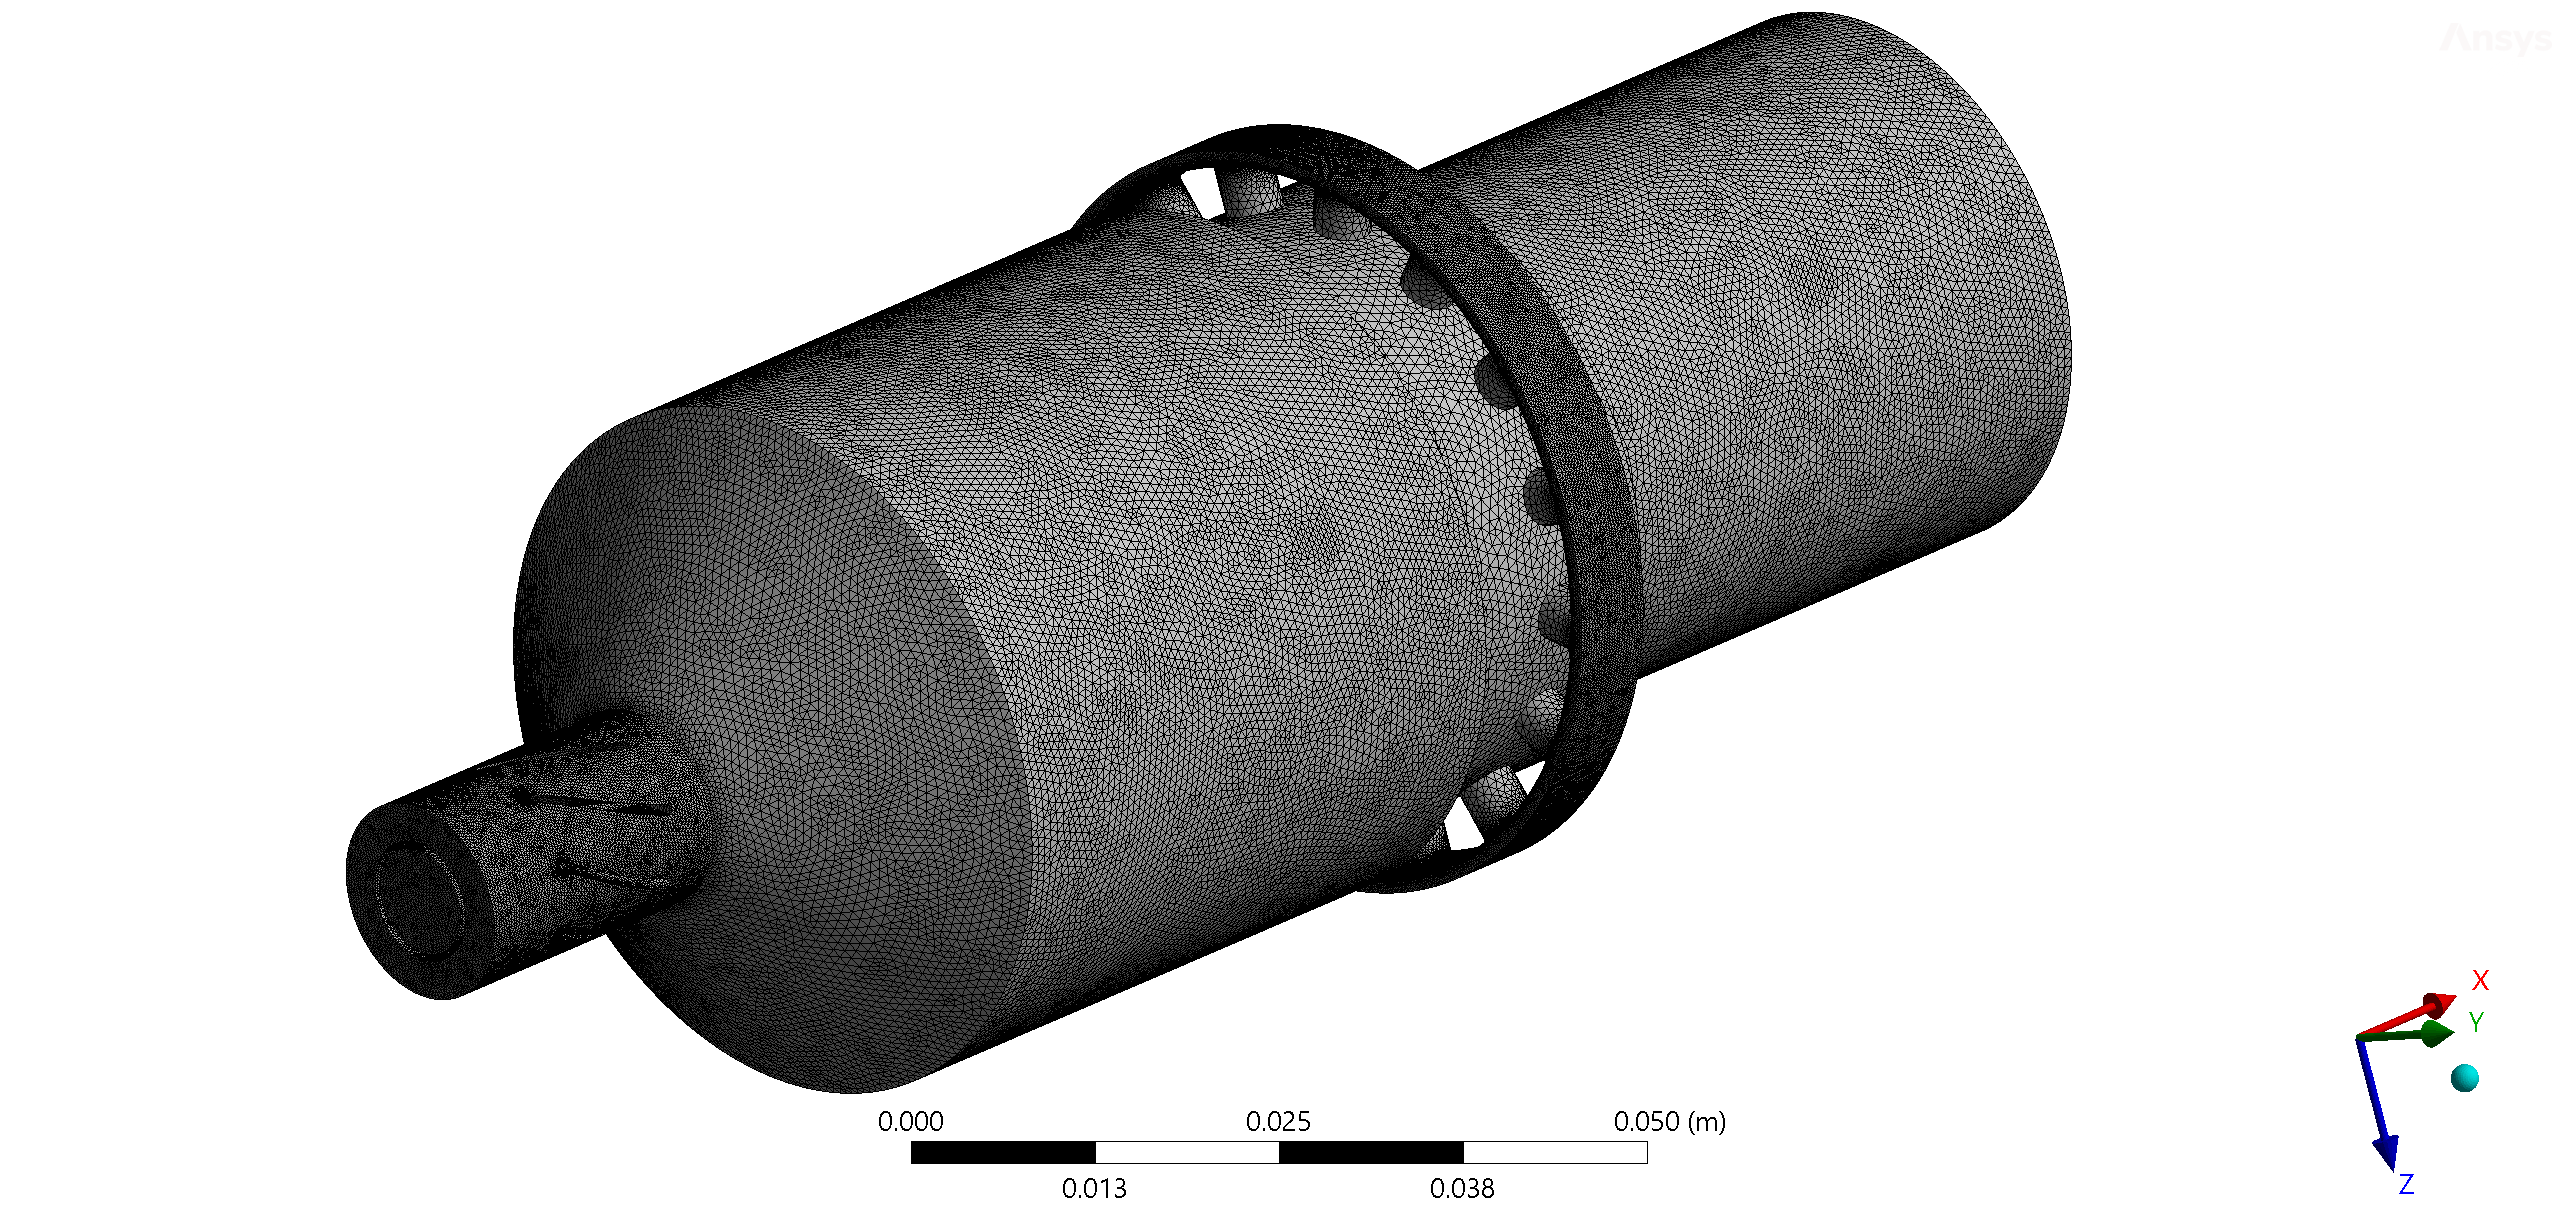
\includegraphics[width=\textwidth]{figs/mesh.png}
    \caption[]%
    {{\small Overall mesh.}}    
\end{subfigure}
\hfill
\begin{subfigure}[b]{0.49\textwidth}   
    \centering 
    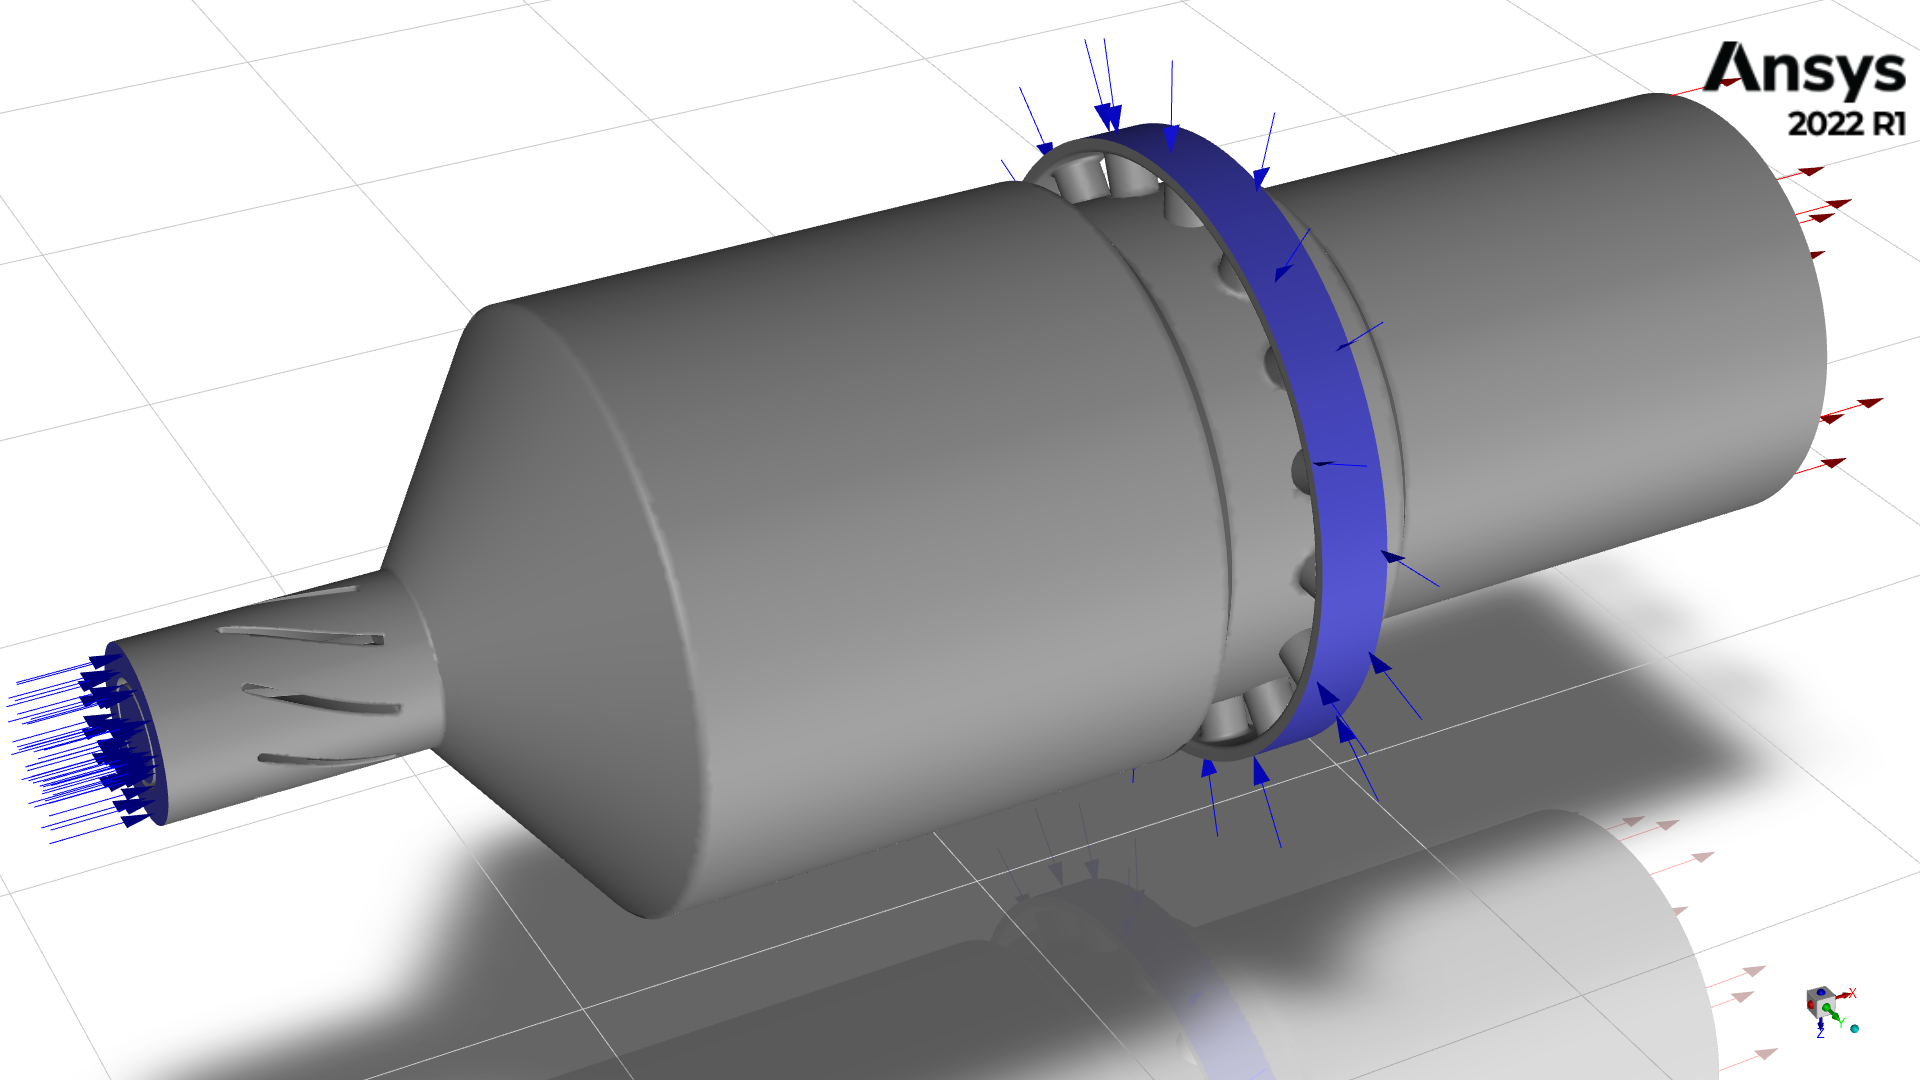
\includegraphics[width=\textwidth]{figs/bound_cond.png}
    \caption[]%
    {{\small Boundary conditions.}}    
\end{subfigure}
\caption{Numerical mesh and setup.} 
\label{fig:numerical_setup}
\end{figure}


\subsubsection{Setup}

To simulate reacting flow, the energy model is turned on. Additionally, the combustion model is set to non-premixed combustion. The settings used are shown in \autoref{fig:setups_lol}. 


\begin{figure}[H]
\centering
\begin{subfigure}[b]{0.49\textwidth}   
    \centering 
    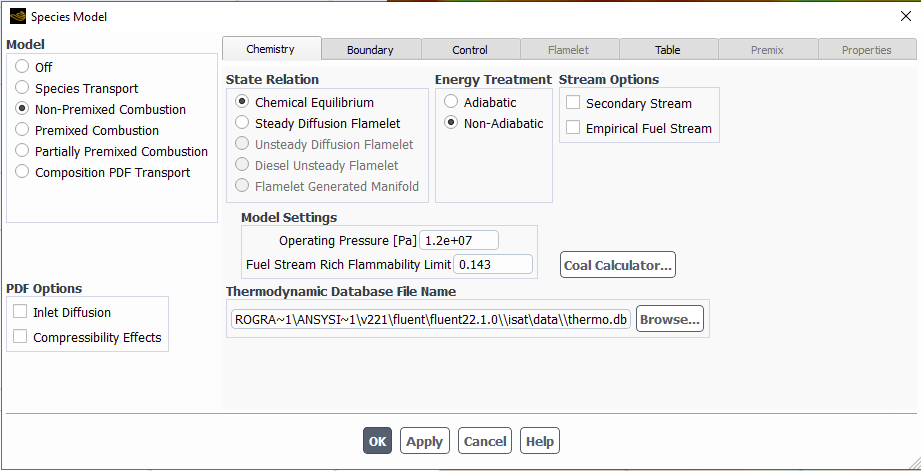
\includegraphics[width=\textwidth]{figs/setup_1.png}
    \caption[]%
    {{\small Setup for chemistry.}}    
\end{subfigure}
\hfill
\begin{subfigure}[b]{0.49\textwidth}   
    \centering 
    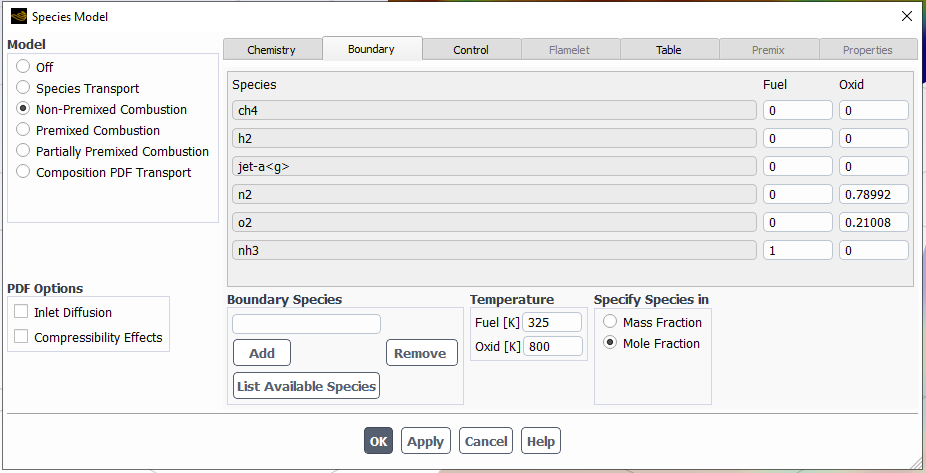
\includegraphics[width=\textwidth]{figs/setup_2.png}
    \caption[]%
    {{\small Setup for boundary.}}    
\end{subfigure}
\caption{Non-Premixed combustion setup.} 
\label{fig:setups_lol}
\end{figure}



\section{Results and discussion}
The following subsections present the results only. The results have been discussed in a later section.

\subsection{Cantera}

The results for the rich zone are presented below generated using the \textit{report} method in cantera:

\clearpage

\begin{minted}[frame=lines,fontsize=\footnotesize,linenos, baselinestretch=1.0]{bash}
Phi=1.24: Outlet temperature = 2217.4 K

  gas:

       temperature   2217.4 K
          pressure   1.2e+06 Pa
           density   1.5189 kg/m^3
  mean mol. weight   23.336 kg/kmol
   phase of matter   gas

                          1 kg             1 kmol     
                     ---------------   ---------------
          enthalpy             41090        9.5886e+05  J
   internal energy       -7.4898e+05       -1.7478e+07  J
           entropy             10359        2.4173e+05  J/K
    Gibbs function       -2.2929e+07       -5.3507e+08  J
 heat capacity c_p            1758.2             41028  J/K
 heat capacity c_v            1401.9             32714  J/K

                      mass frac. Y      mole frac. X     chem. pot. / RT
                     ---------------   ---------------   ---------------
                N2           0.76963           0.73853            -24.18
                 H        1.8748e-09        4.9999e-08           -14.749
                O2           0.12591           0.10578           -27.926
                OH        0.00012524        0.00019796           -28.716
                 O        1.9361e-06         3.253e-06            -13.96
                H2        1.6296e-07         2.173e-06           -29.498
               H2O           0.10401            0.1552           -43.471
               HO2         1.016e-06        8.2747e-07           -42.678
              H2O2        1.1488e-07        9.0793e-08           -57.432
                NO        0.00031302        0.00028043           -27.924
\end{minted}

The results after the lean region, i.e. the combustor outlet are presented below:

\begin{minted}[frame=lines,fontsize=\footnotesize,linenos, baselinestretch=1.0]{shell}
Phi=0.42: Outlet temperature = 1675.5 K

  gas:

       temperature   1675.5 K
          pressure   1.2e+06 Pa
           density   2.3156 kg/m^3
  mean mol. weight   26.882 kg/kmol
   phase of matter   gas

                          1 kg             1 kmol     
                     ---------------   ---------------
          enthalpy        3.4244e+05        9.2055e+06  J
   internal energy       -1.7579e+05       -4.7255e+06  J
           entropy            8732.5        2.3475e+05  J/K
    Gibbs function       -1.4289e+07       -3.8411e+08  J
 heat capacity c_p            1399.2             37614  J/K
 heat capacity c_v            1089.9             29299  J/K

                      mass frac. Y      mole frac. X     chem. pot. / RT
                     ---------------   ---------------   ---------------
                N2           0.77429           0.64498           -25.251
                 H        2.0651e-05        0.00047808           -9.9996
                O2        3.0781e-06        2.2448e-06           -39.673
                OH        0.00022282        0.00030573           -29.836
                 O        9.0035e-07        1.3132e-06           -19.836
                H2         0.0060517           0.07005           -19.999
               H2O           0.21935           0.28413           -39.836
               HO2        5.1905e-09        3.6697e-09           -49.673
              H2O2          7.66e-09        5.2552e-09           -59.672
                NO         5.847e-05        4.5472e-05           -32.309
                
NOx at outlet: 58.47 ppm
\end{minted}

\subsection{Simulation}

Analyzing the velocity field is essential, as it directly influences flame length, fuel-air mixing quality, and residence time within the combustion chamber—all of which affect combustion stability and \ce{NOx} formation. The profiles show the effectiveness of the swirlers in mixing the fuel with the air. This can be further seen when the species mass fractions are presented.

\begin{figure}[H]
\centering
\begin{subfigure}[b]{0.49\textwidth}   
    \centering 
    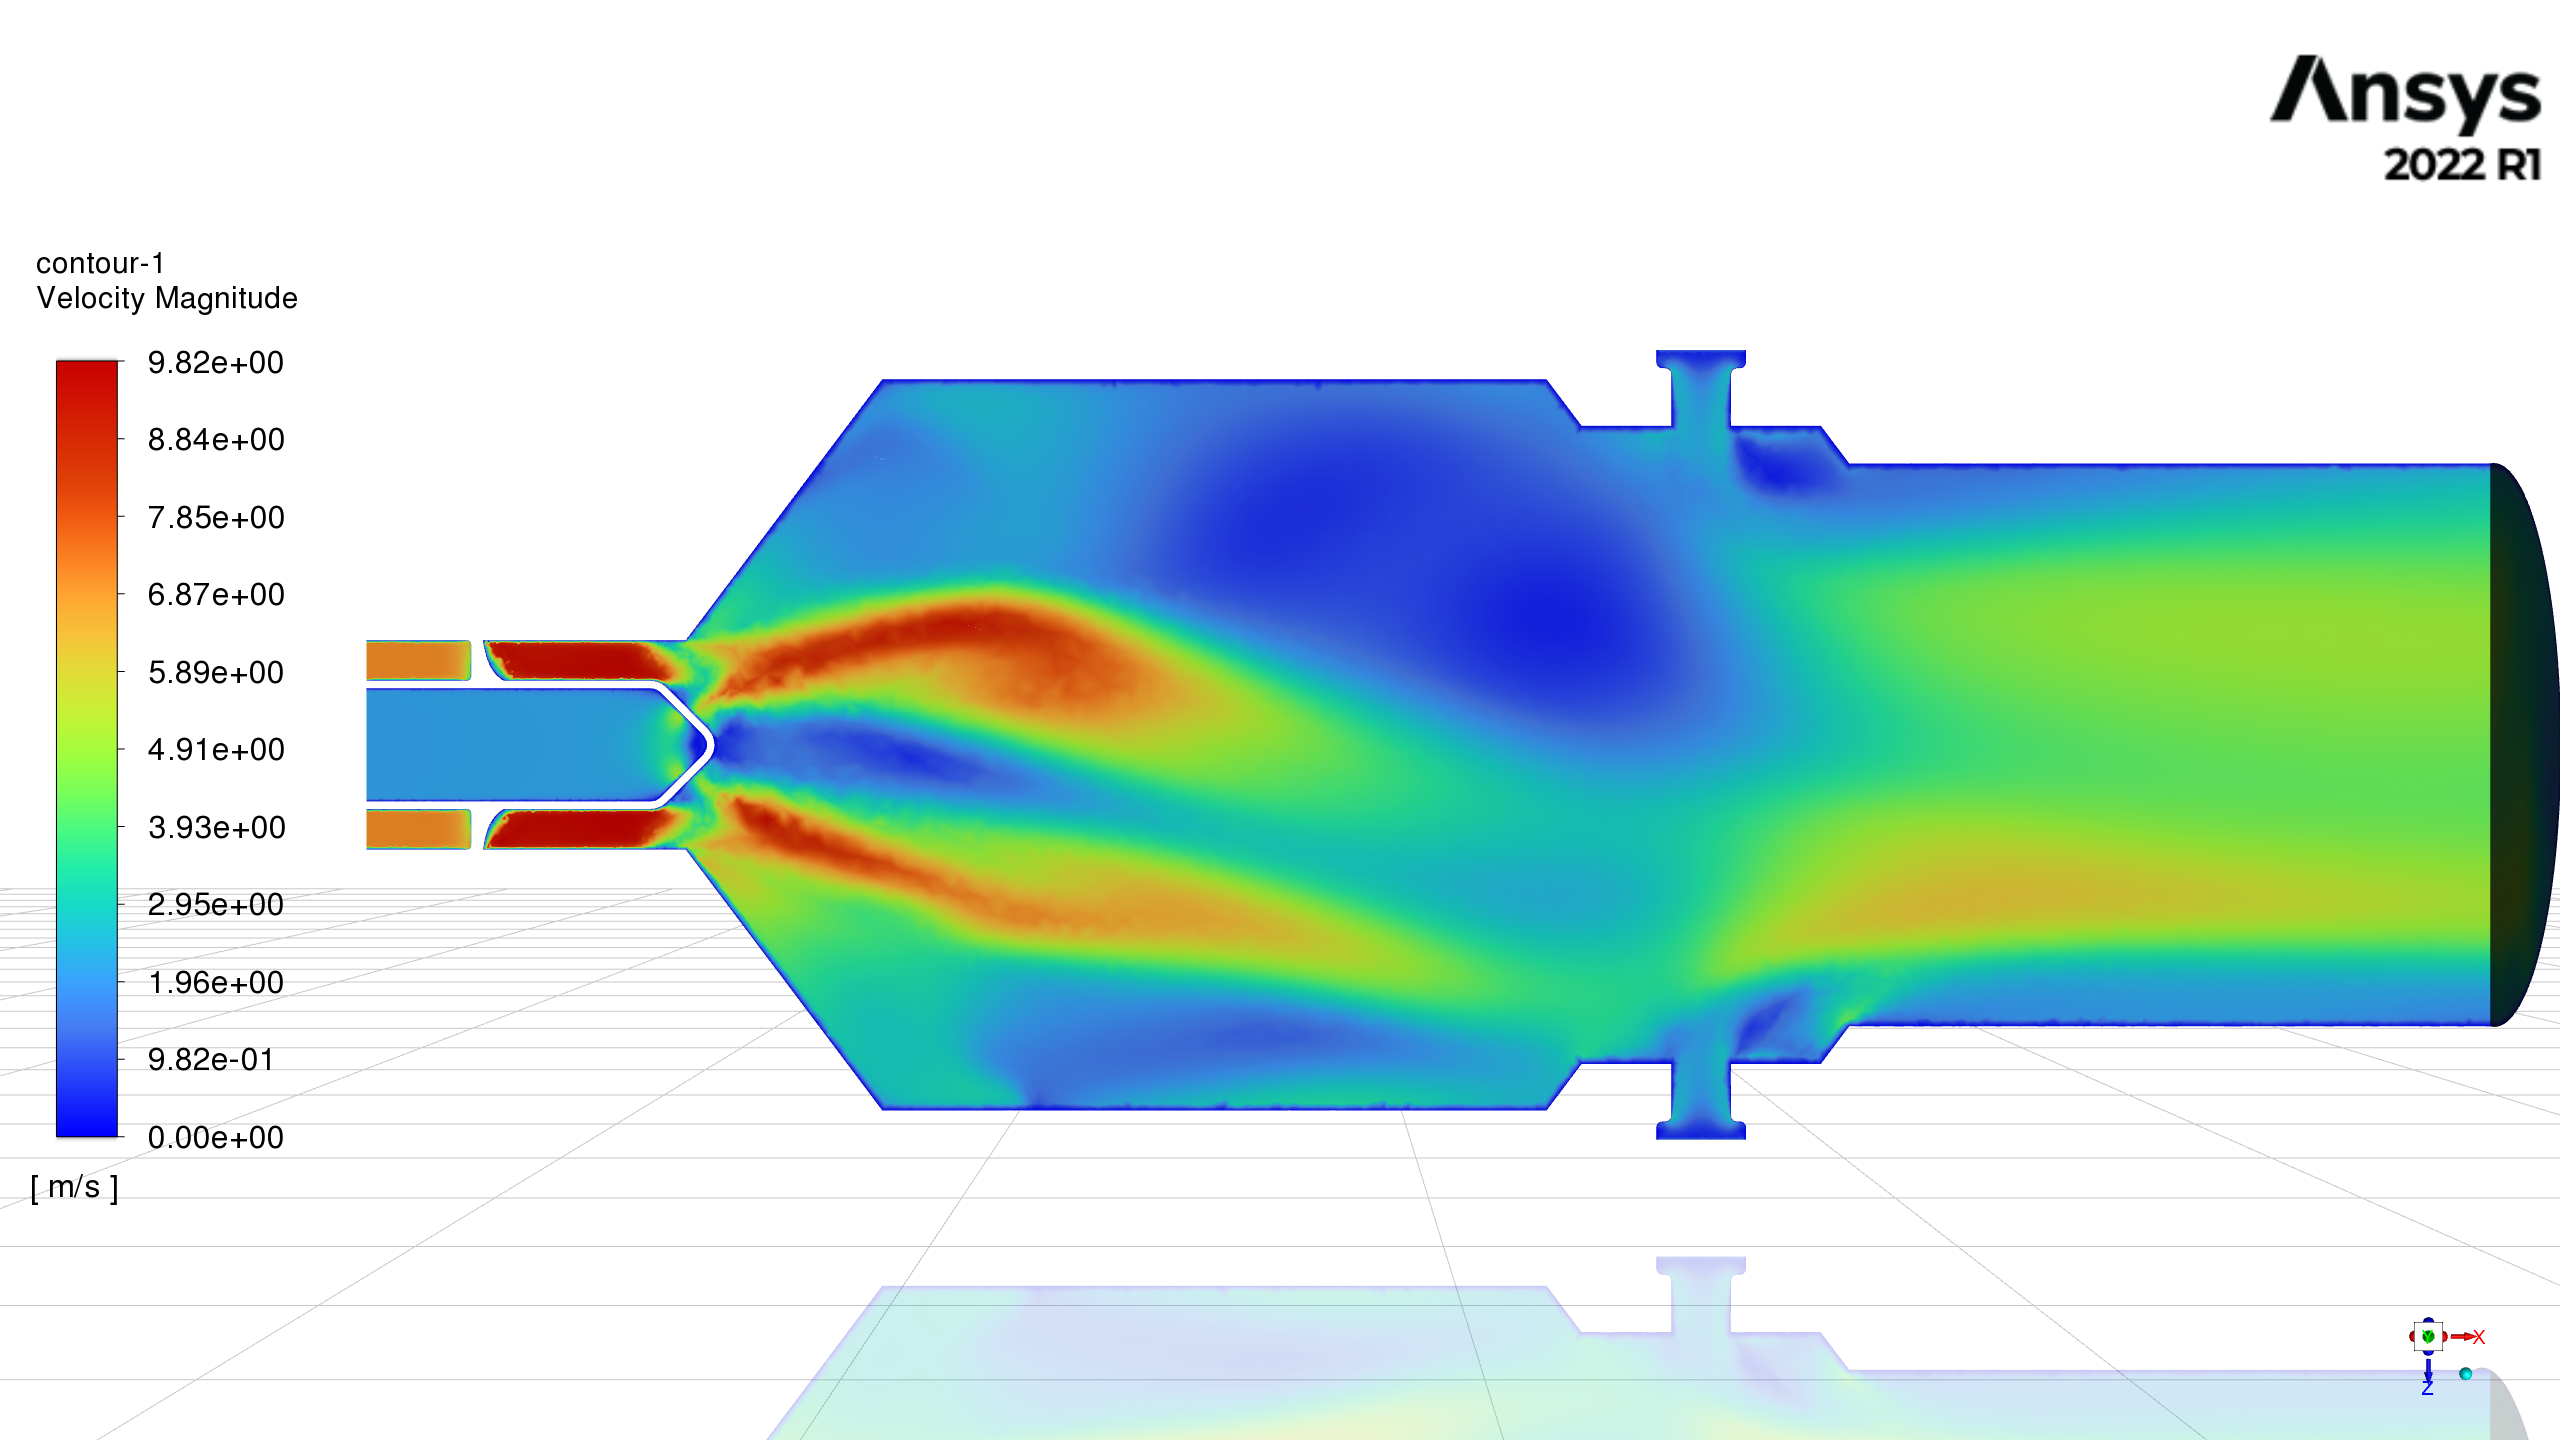
\includegraphics[width=\textwidth]{figs/velocity.png}
\end{subfigure}
\hfill
\begin{subfigure}[b]{0.49\textwidth}   
    \centering 
    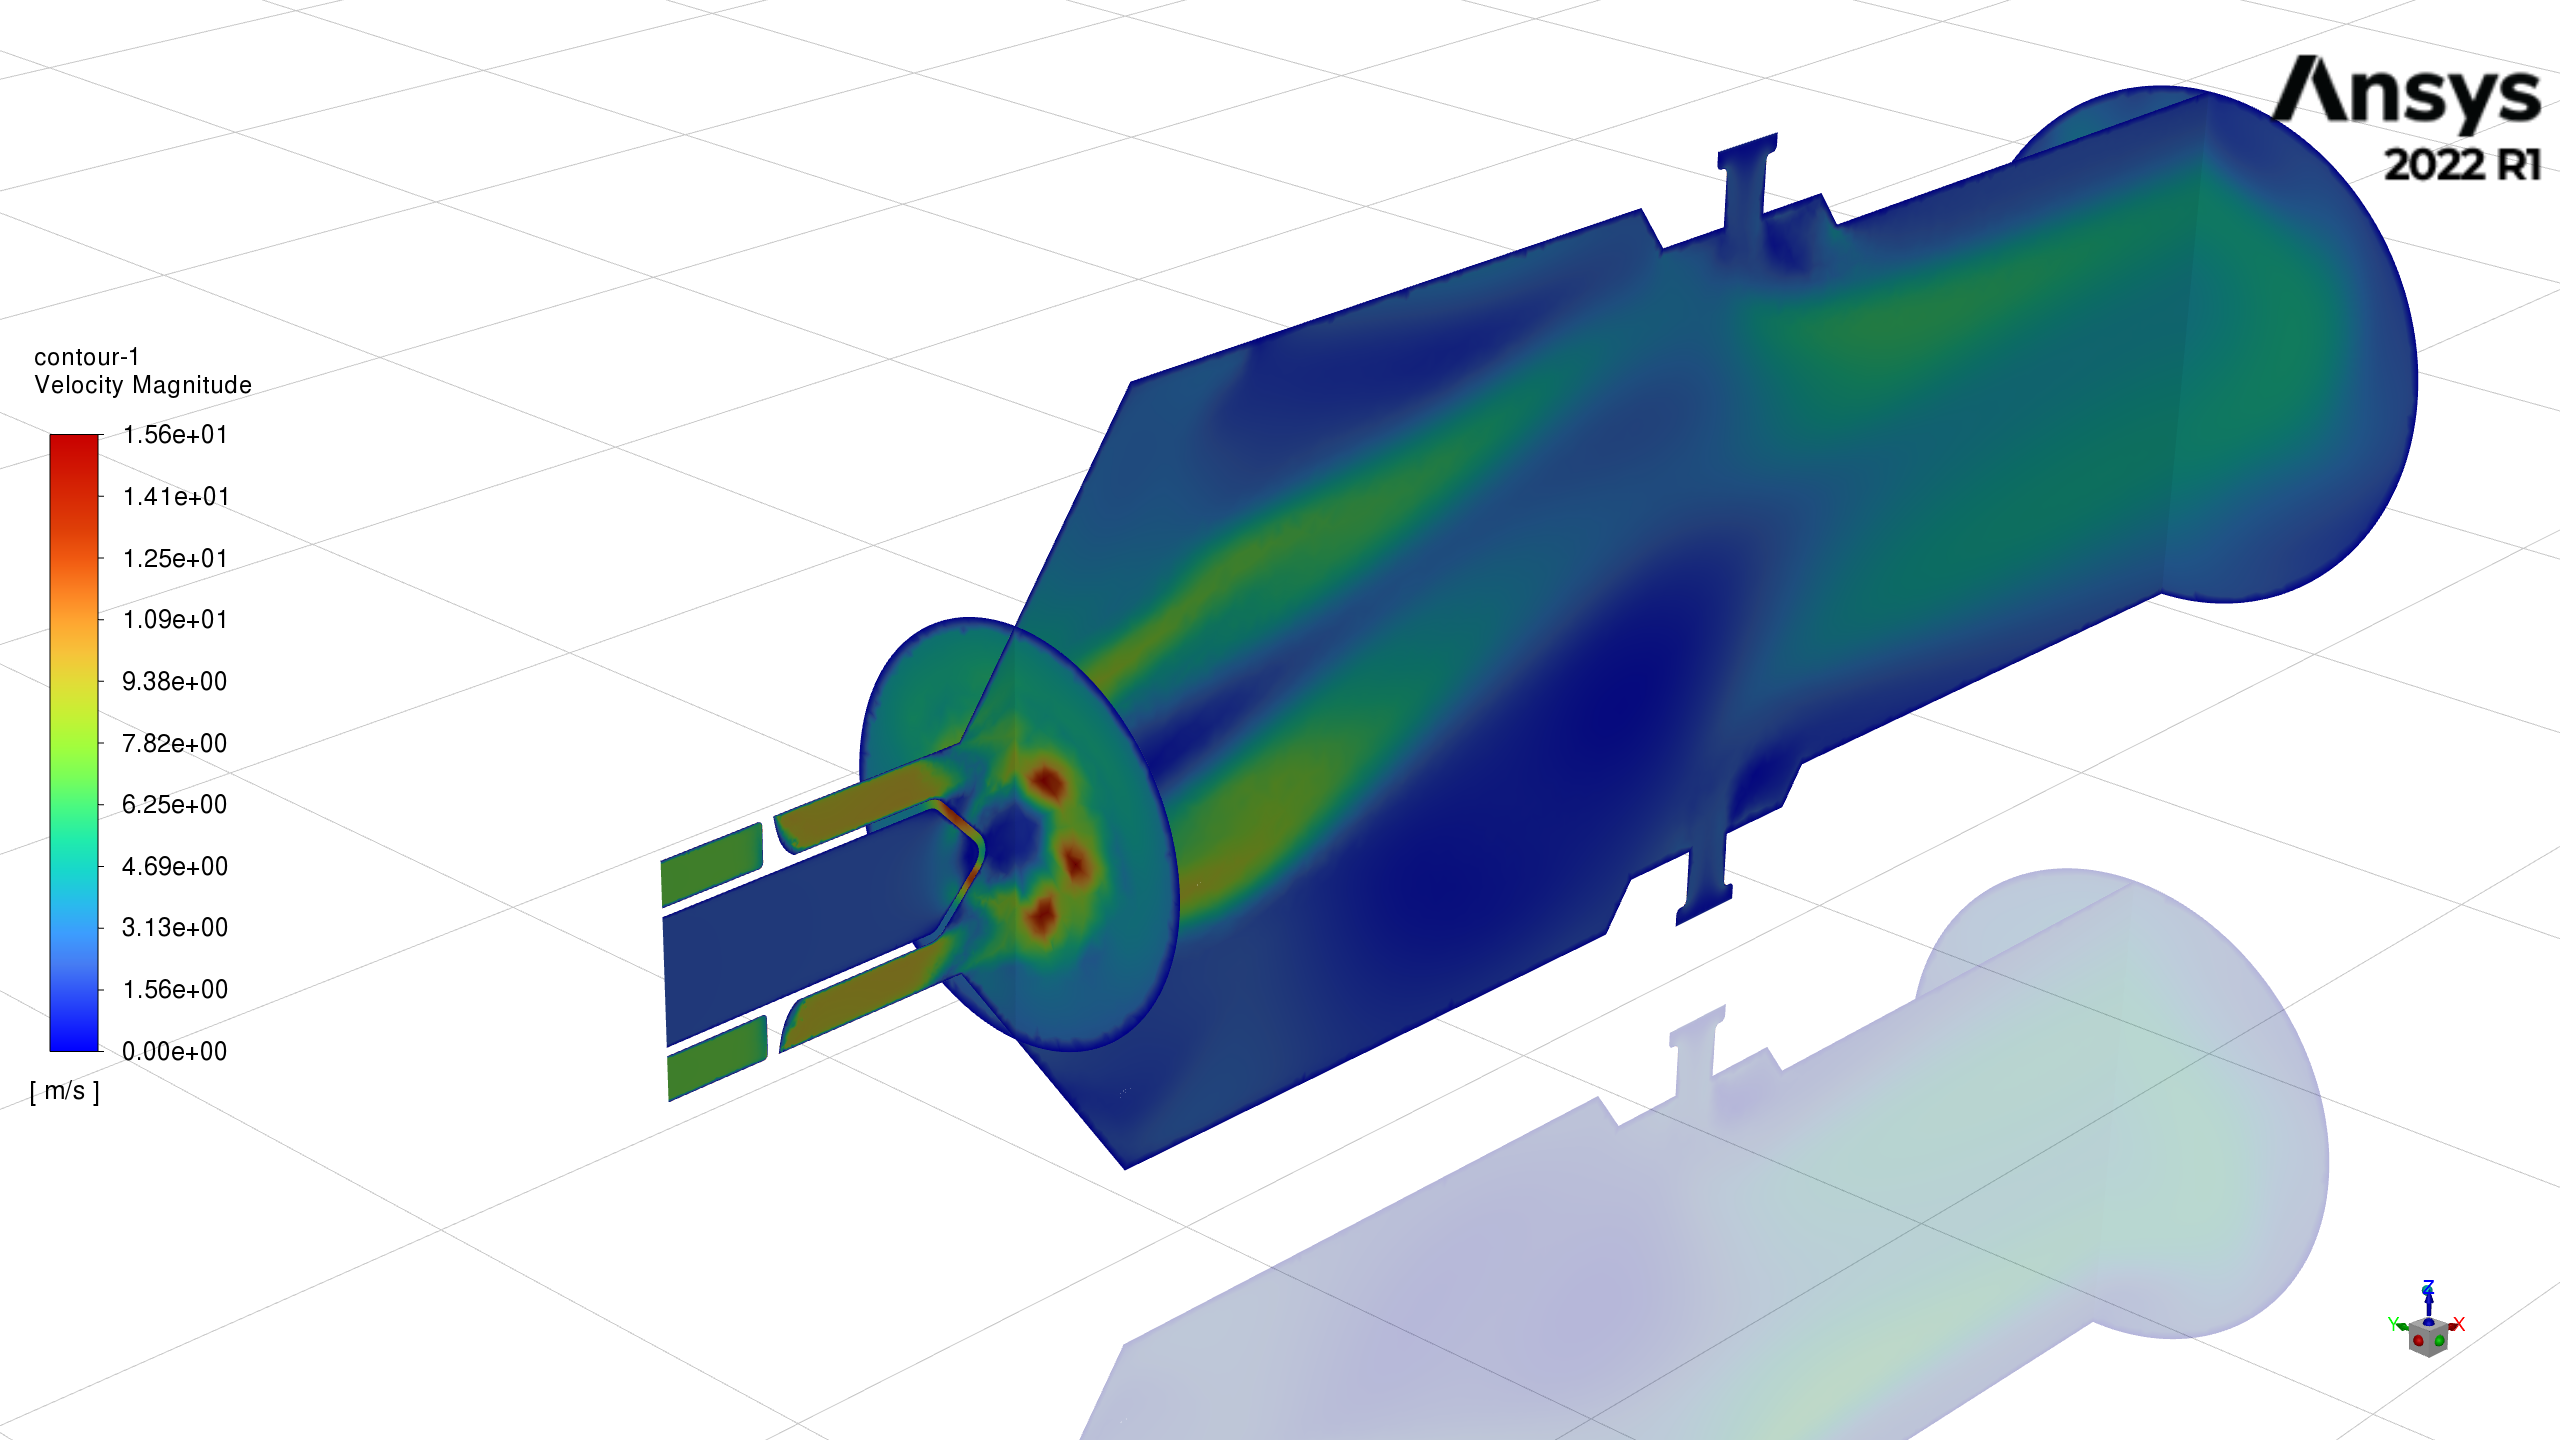
\includegraphics[width=\textwidth]{figs/velocity_front.png}
\end{subfigure}
\caption{Velocity profile for the combustor.} \label{fig:velocity_field}
\end{figure}


One of the most important factors that determines the success of the injector is the temperature of the mixture in the combustion system, as it is the only factor responsible for the production of \ce{NOx}. We know that \ce{NOx} is being produced when the flame is above 1850 K. The temperatures within combustor reach around 2300 K. This indicates that \ce{NOx} are being produced. However, as the cooling air is added, the temperature drops, neutralizing the radicals responsible for emissions. One can look at the mass fraction of \ce{NO} to calculate the the amount of emissions being produced. This will be seen when the species are discussed.

\begin{figure}[H]
\centering
\begin{subfigure}[b]{0.49\textwidth}   
    \centering 
    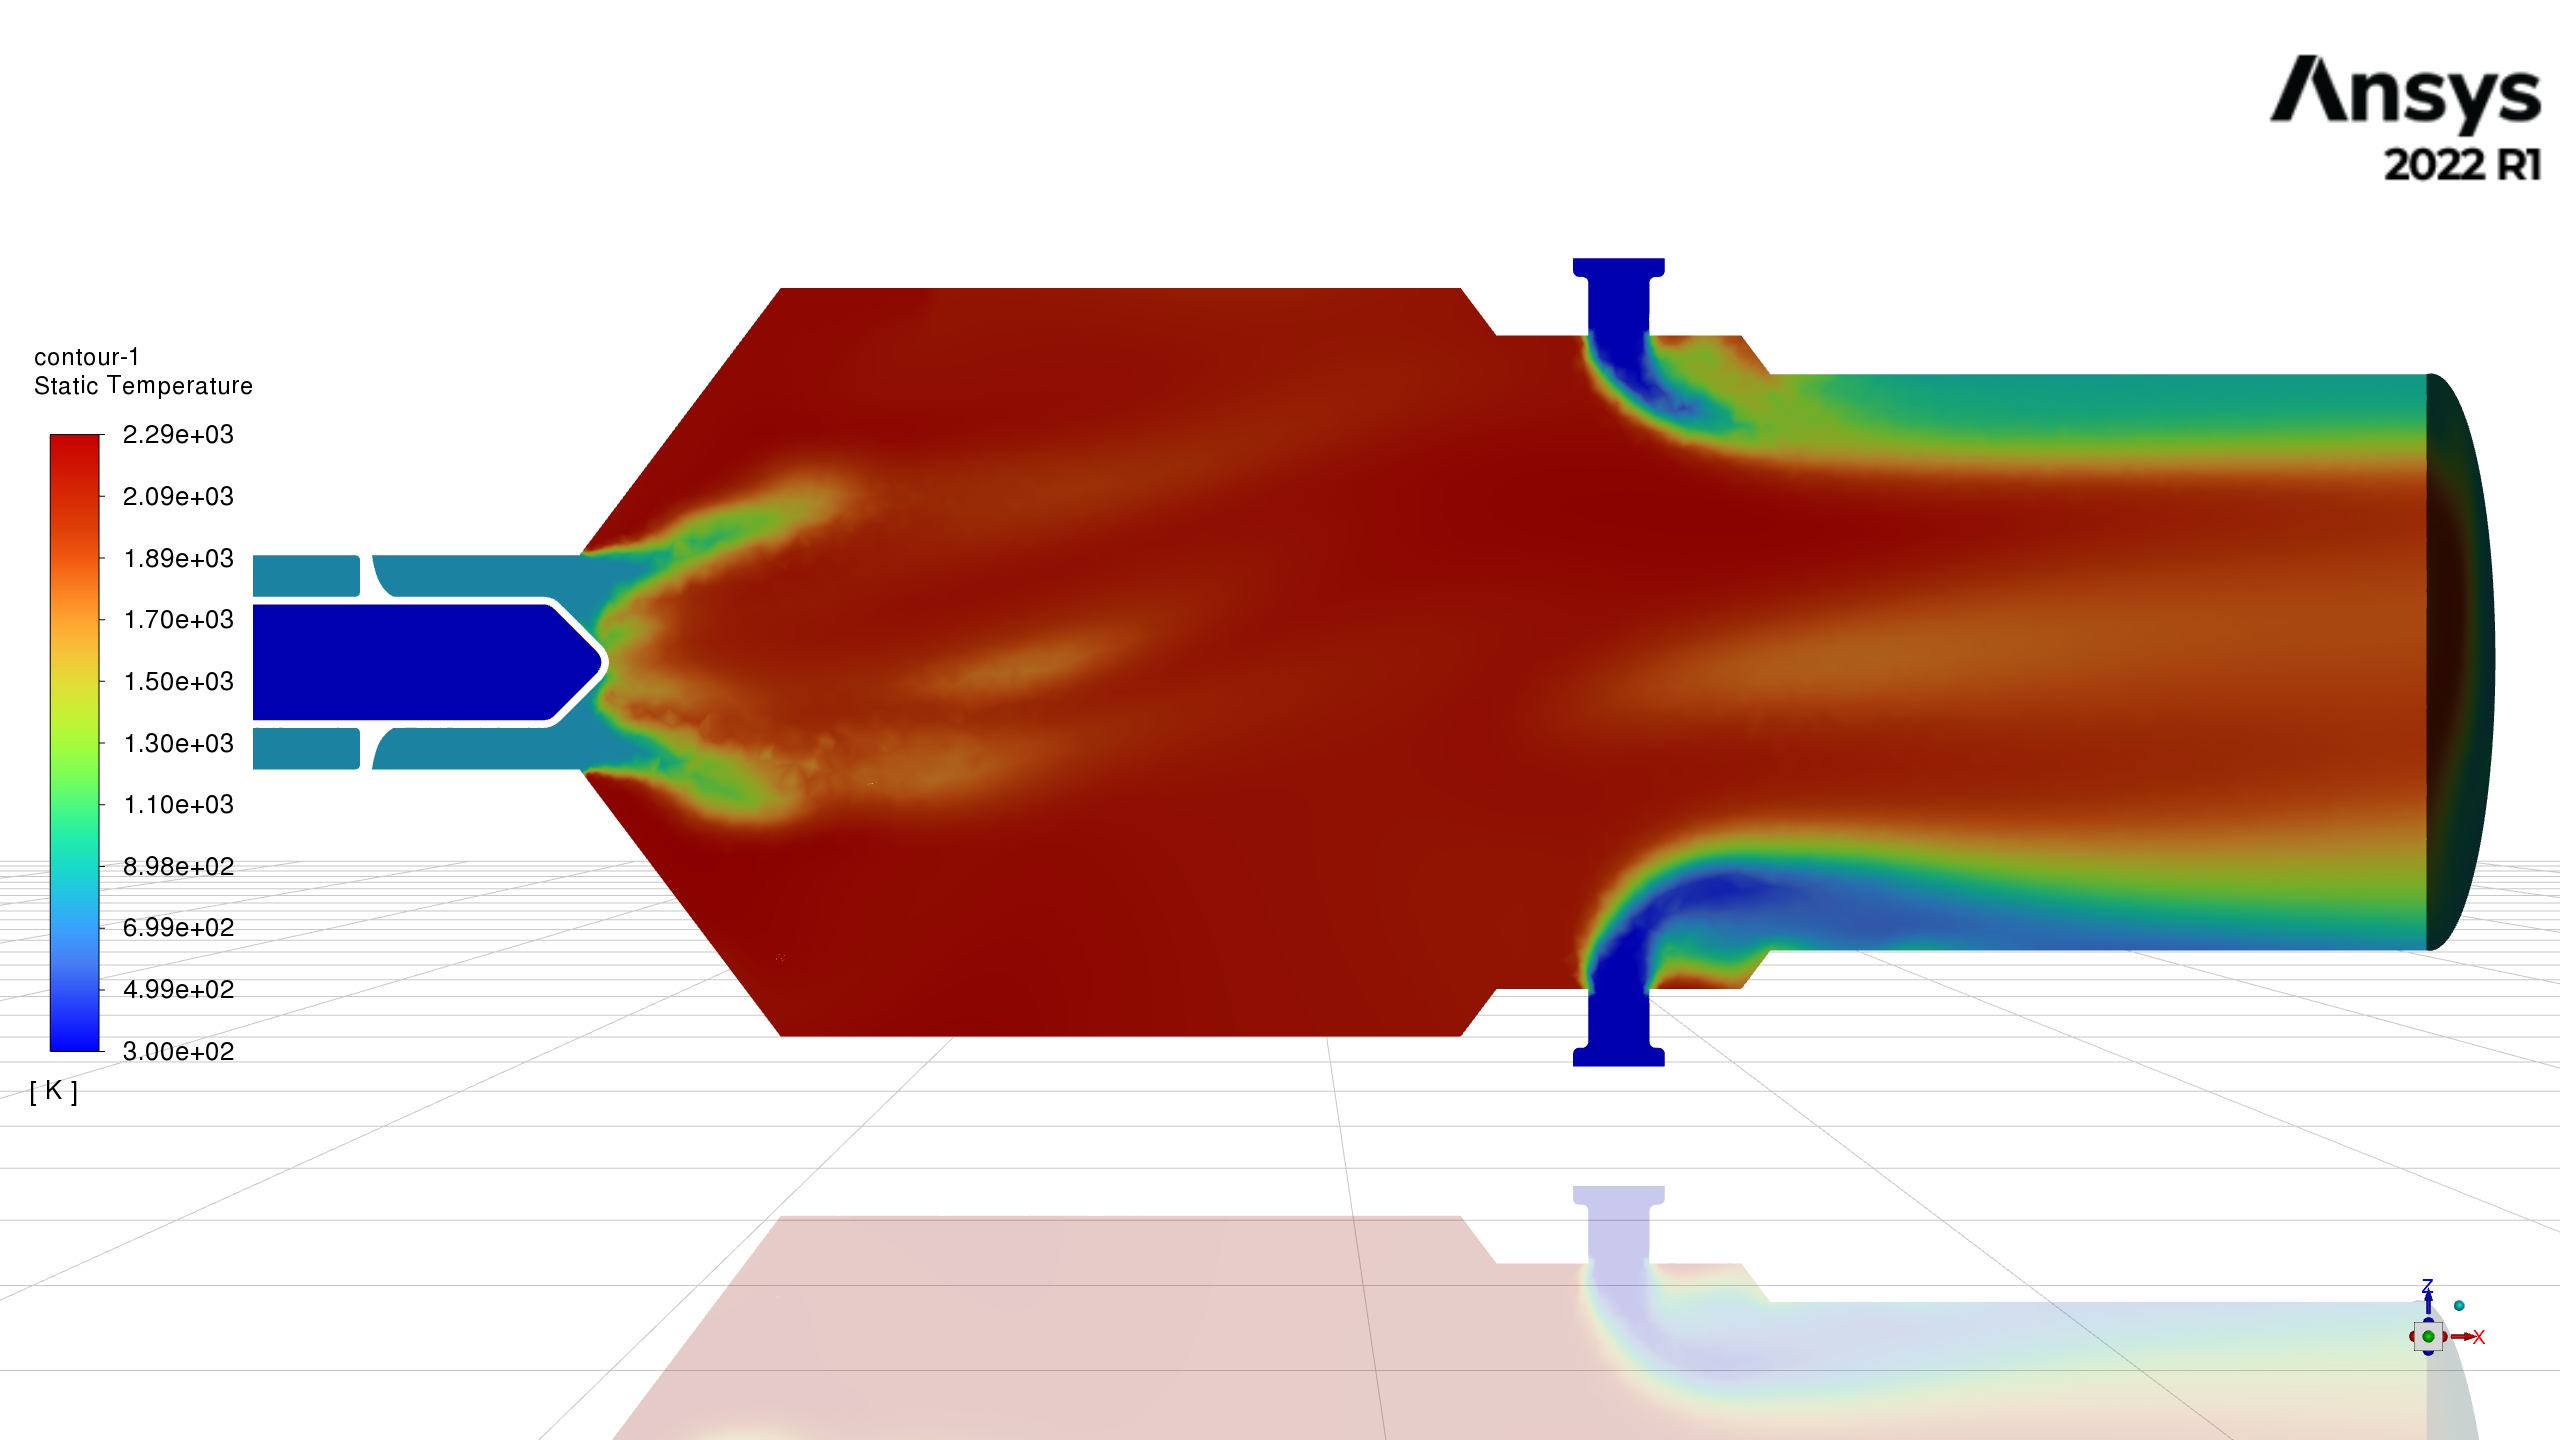
\includegraphics[width=\textwidth]{figs/temperature.png}
\end{subfigure}
\hfill
\begin{subfigure}[b]{0.49\textwidth}   
    \centering 
    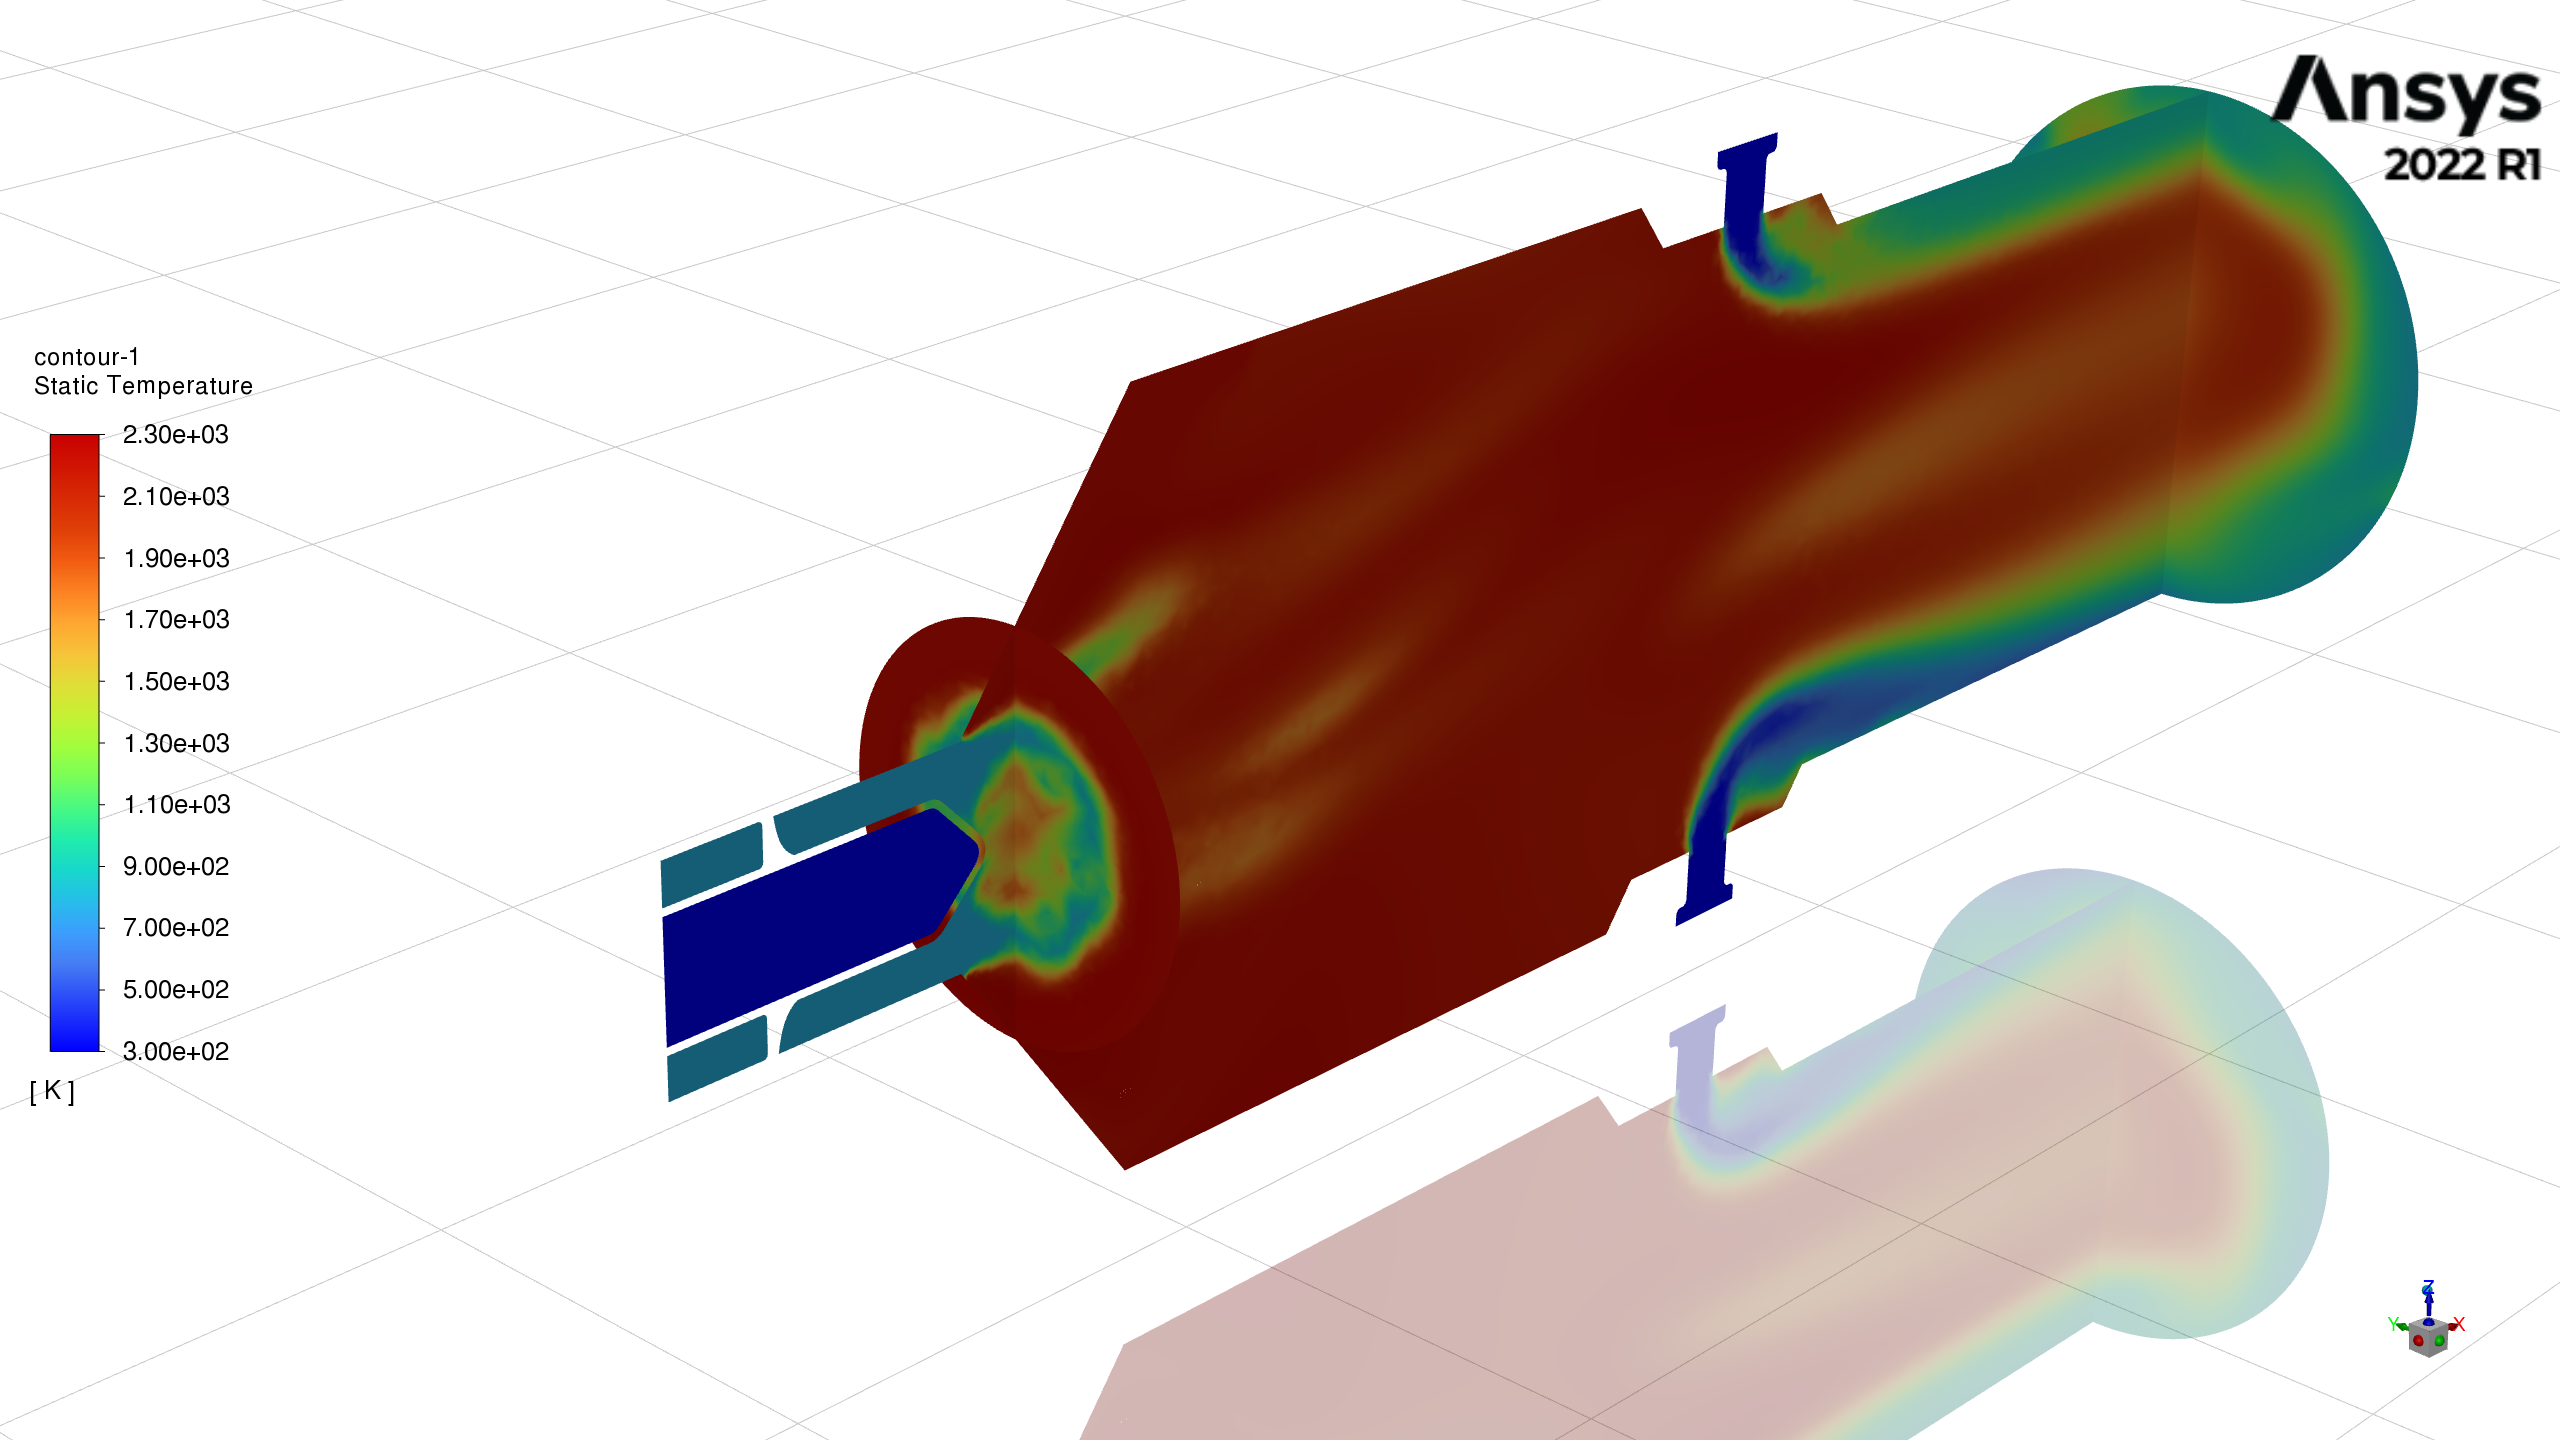
\includegraphics[width=\textwidth]{figs/pressure_front.png}
\end{subfigure}
\caption{Numerical mesh and setup.} \label{fig:numerical_setup}
\end{figure}


\autoref{fig:nh3species} shows the mass fraction of \ce{NH3}. It can be seen that in the fuel inlet, the mass fraction is 1. However, as soon as it mixes with the inlet air, the mass fraction reduces indicating that the NH3 is being consumed as the fuel. \autoref{fig:o2species} shows the mass fraction of \ce{O2}. Initially, it is the highest at the primary air inlet, and then starts being consumed as the oxidizer. However, a rise in the mass fraction can be seen when the secondary air is added.


The hydroxyl radical (\ce{OH}) is a key indicator of combustion activity and is commonly used to visualize flame fronts in reacting flows. Regions of high OH concentration correspond to zones where combustion is actively occurring, making it an effective marker for assessing flame stability and propagation characteristics. From \autoref{fig:ohspecies}, it can be observed that the flames being formed are not concentrated and are occupying the while combustor in the primary zone. This can be due to the fact the the fuel is present in excess allowing the flames to spread out.


Finally, we look at \ce{NOx} in \autoref{fig:nospecies}. It can clearly be seen that in the primary zone, the mass fraction of \ce{NO} is high. It is highly concentrated next to the flame front. However, after the secondary air is added, the mass fraction is reduced and is quite low near the outlet. 

\begin{figure}[H]
    \centering

    \begin{subfigure}[b]{0.49\textwidth}
        \centering
        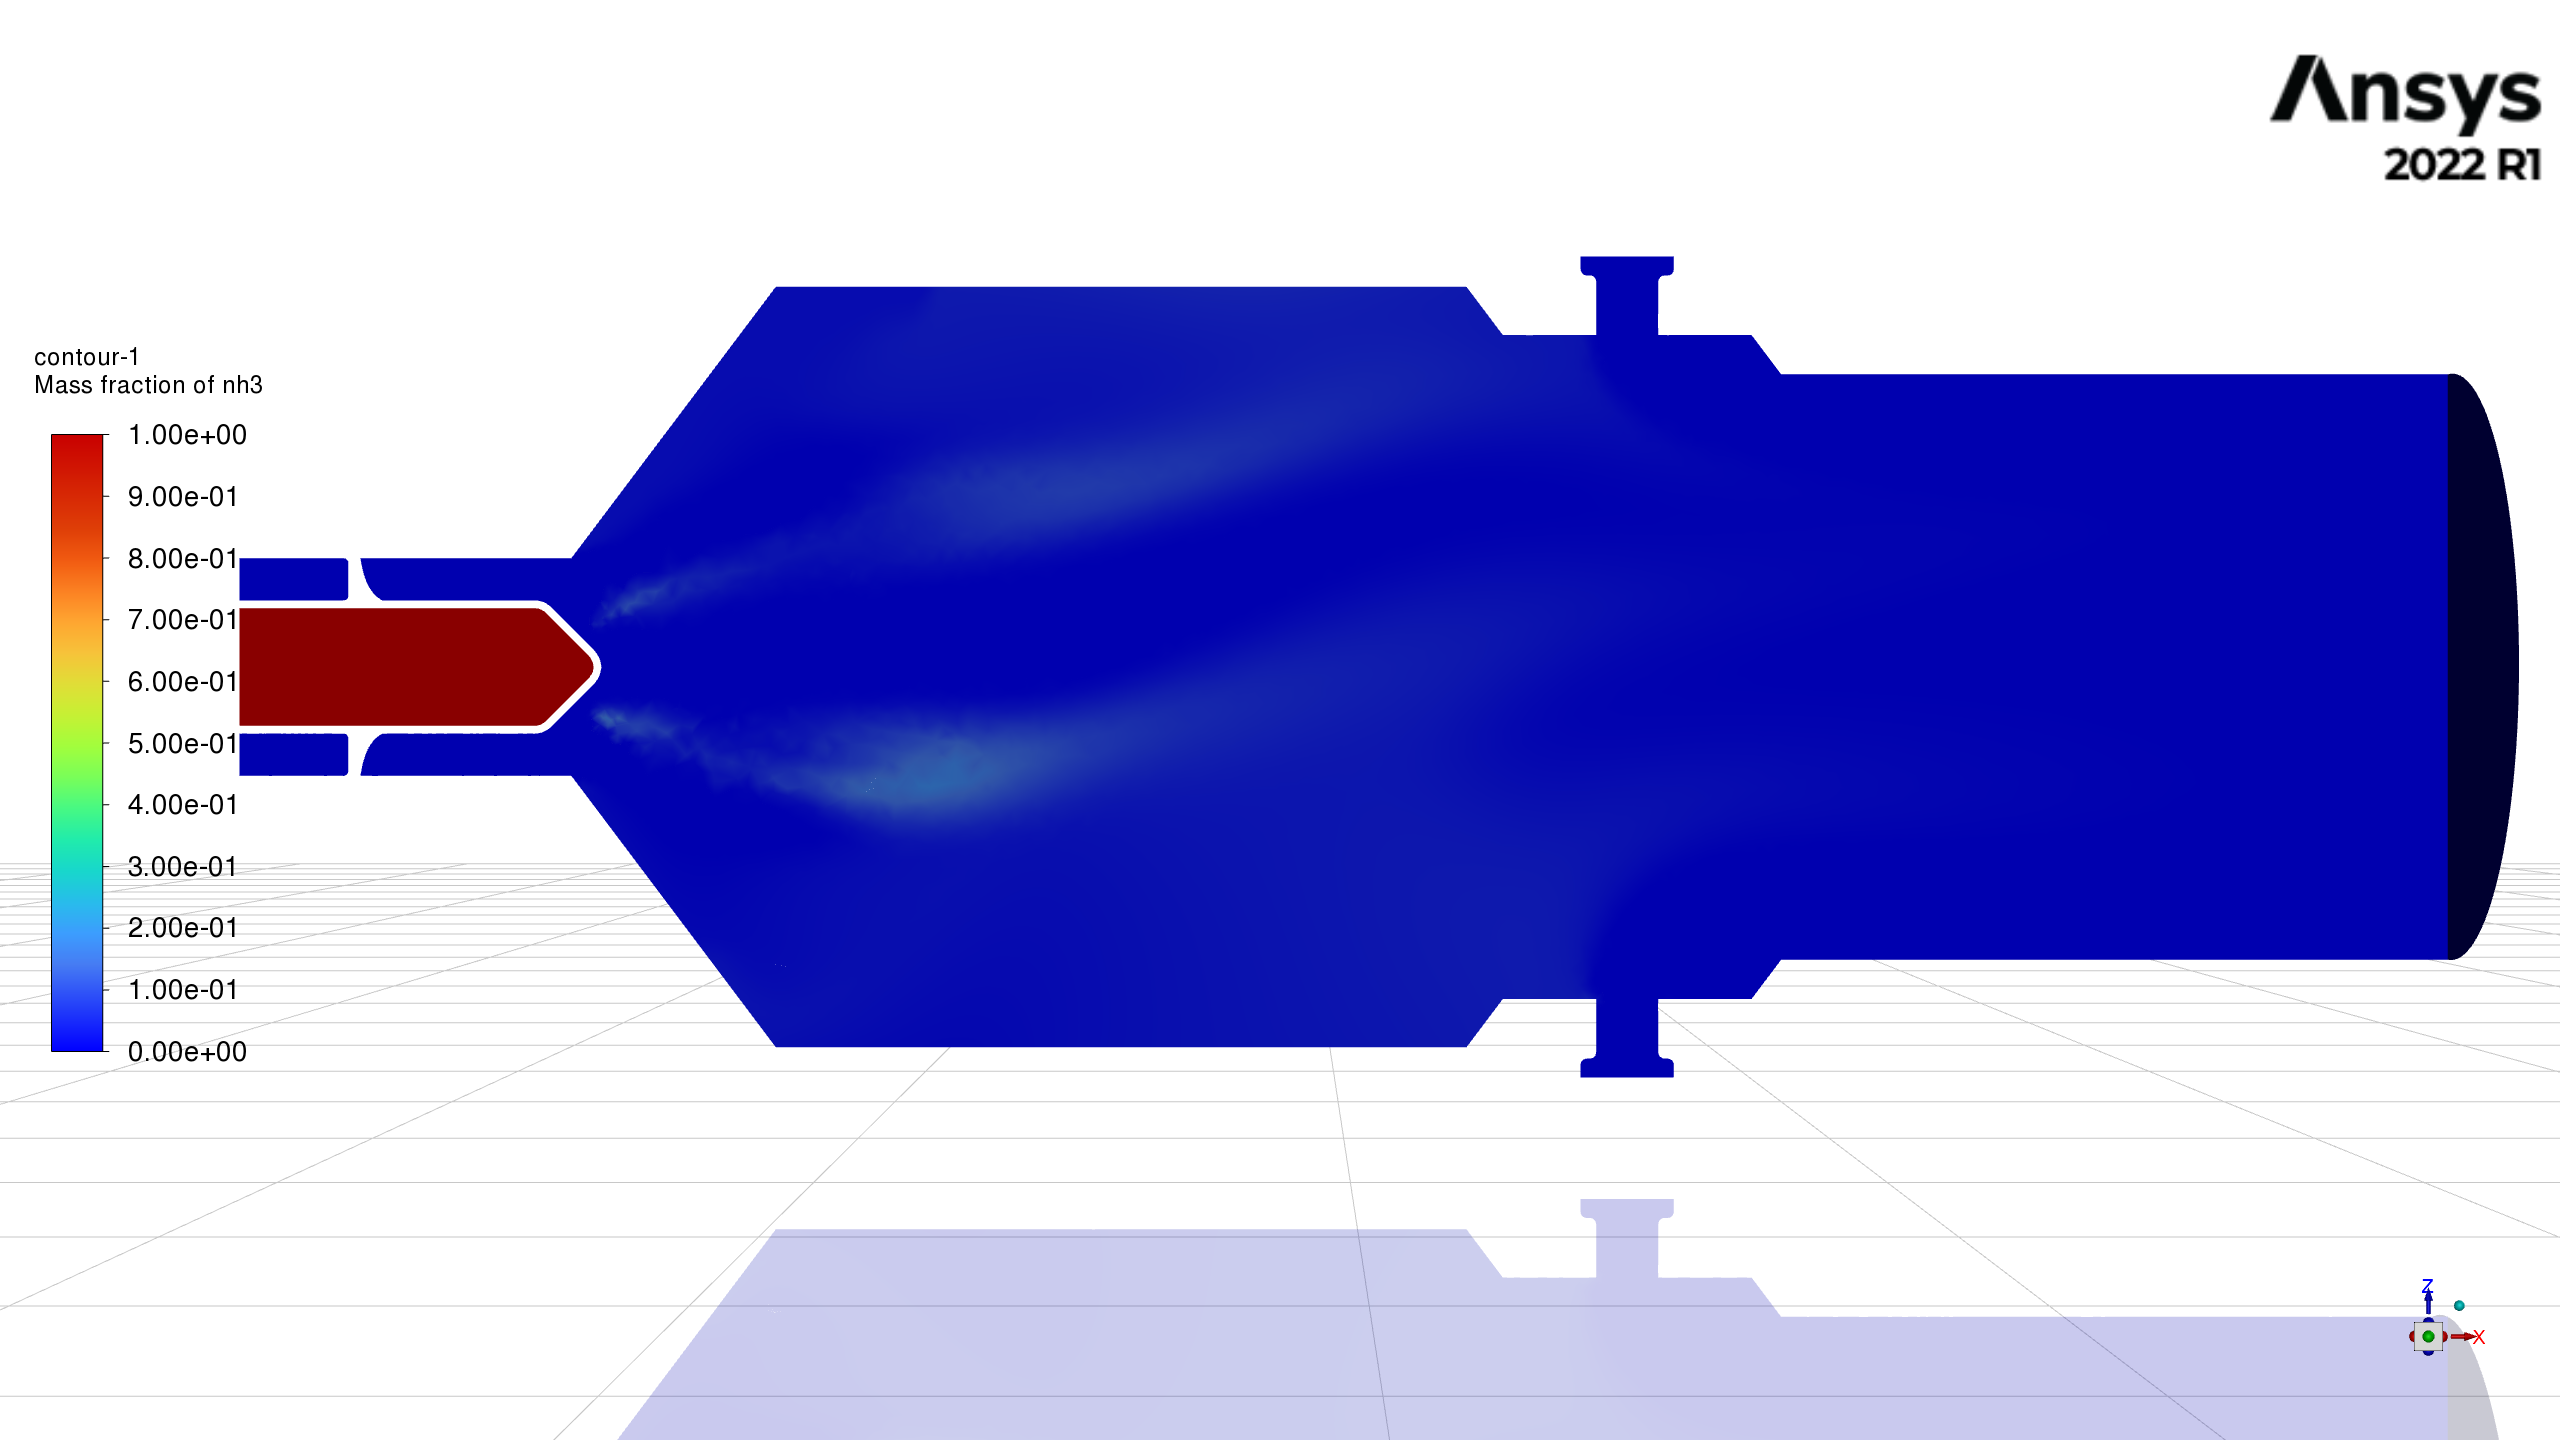
\includegraphics[width=\linewidth]{figs/species_nh3.png}
        \caption{Species \ce{NH3}}\label{fig:nh3species}
    \end{subfigure}
    \hfill
    \begin{subfigure}[b]{0.49\textwidth}
        \centering
        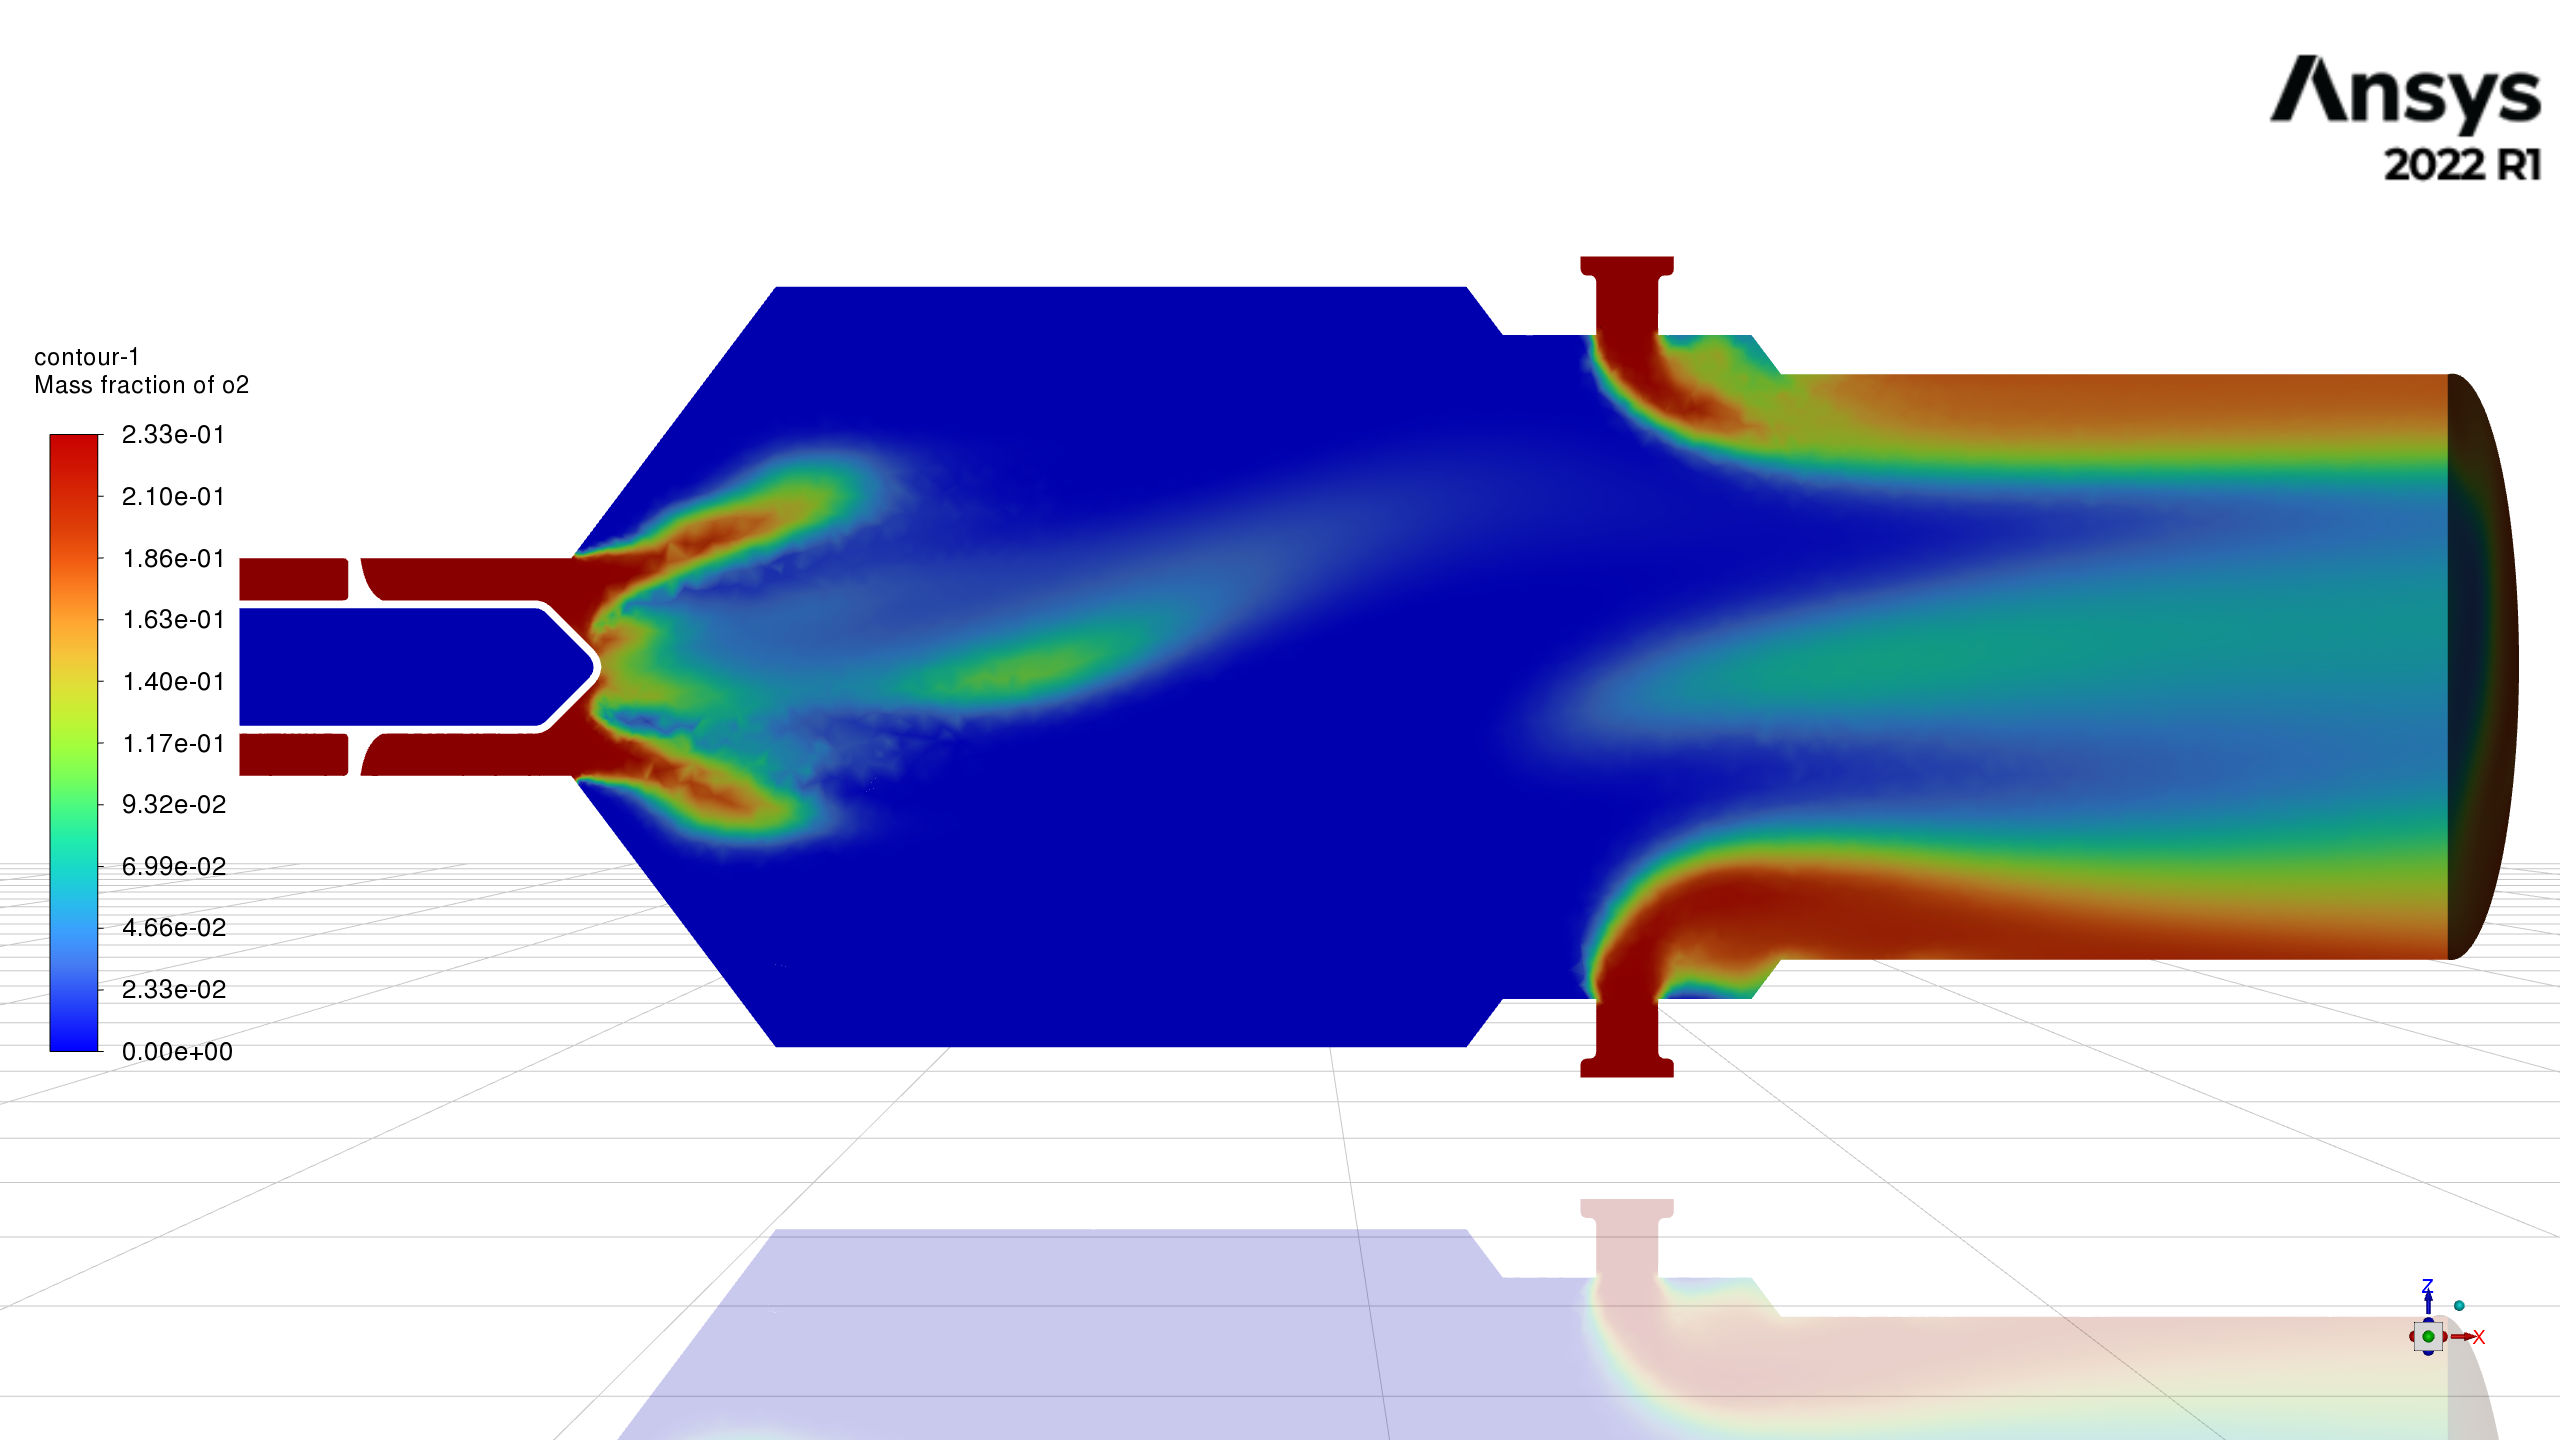
\includegraphics[width=\linewidth]{figs/species_o2.png}
        \caption{Species \ce{O2}}\label{fig:o2species}
    \end{subfigure}

    \vspace{0.5cm}

    \begin{subfigure}[b]{0.49\textwidth}
        \centering
        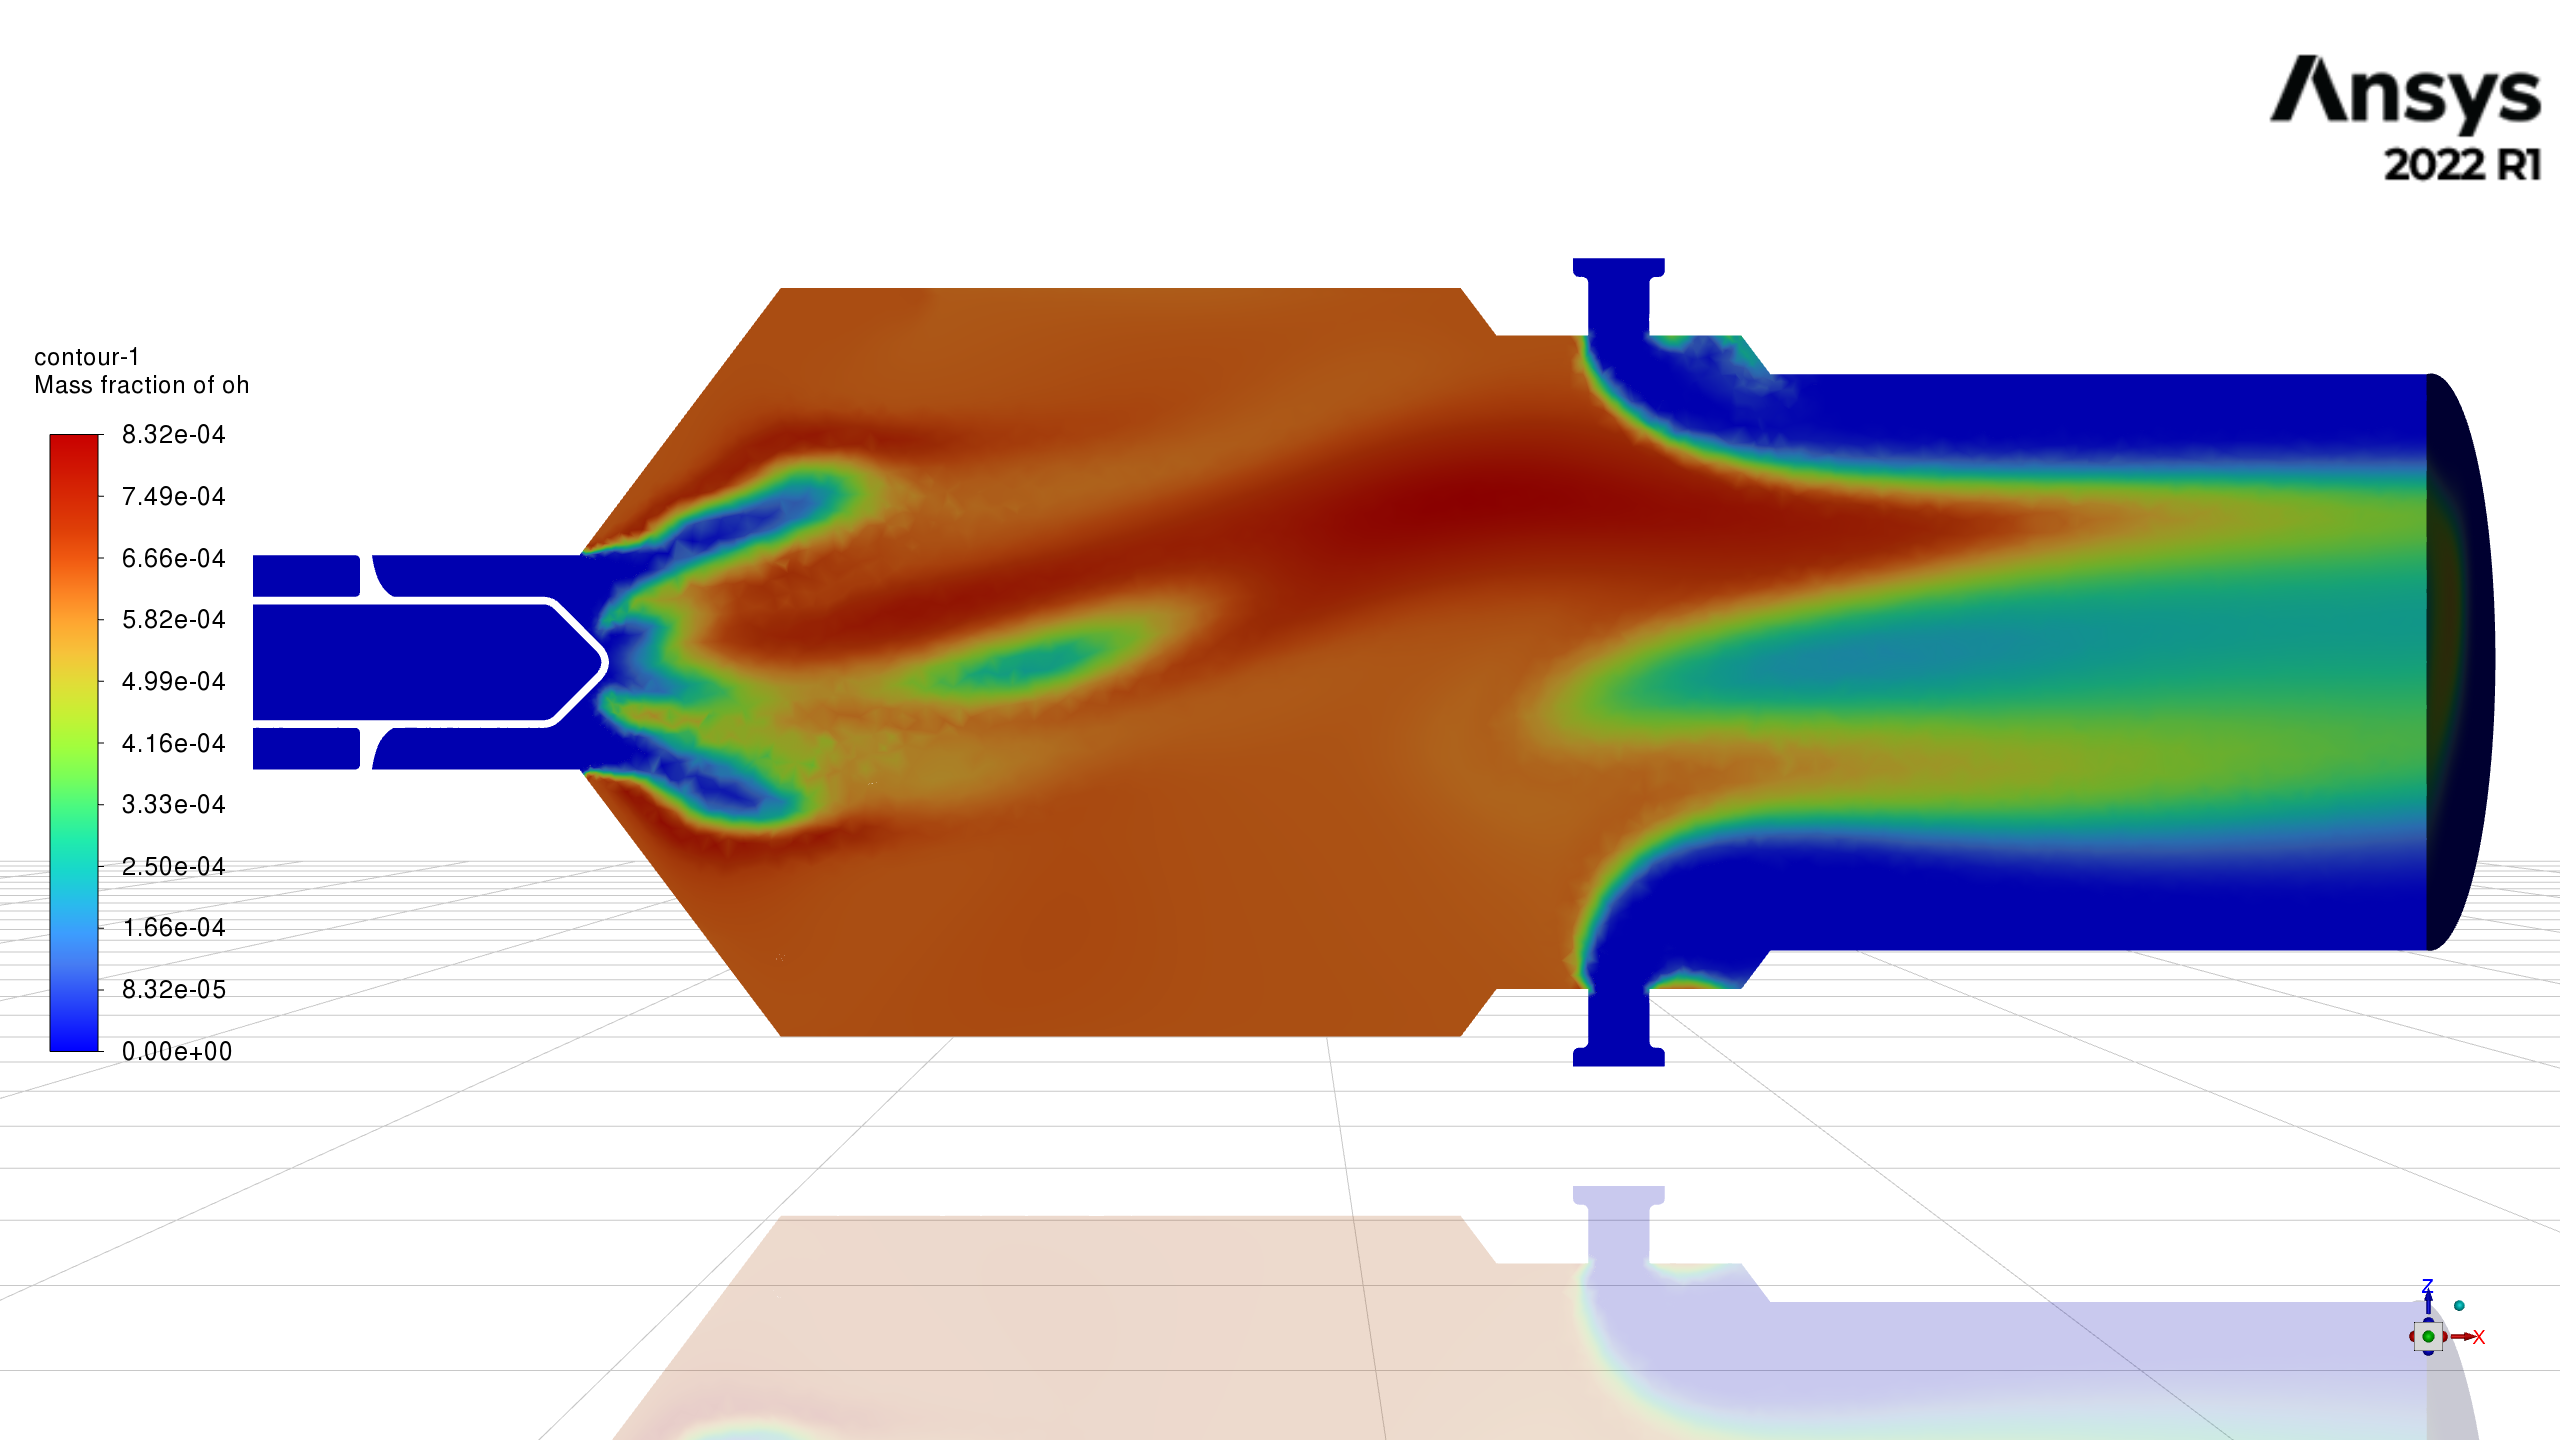
\includegraphics[width=\linewidth]{figs/species_oh.png}
        \caption{Species \ce{OH}}\label{fig:ohspecies}
    \end{subfigure}
    \hfill
    \begin{subfigure}[b]{0.49\textwidth}
        \centering
        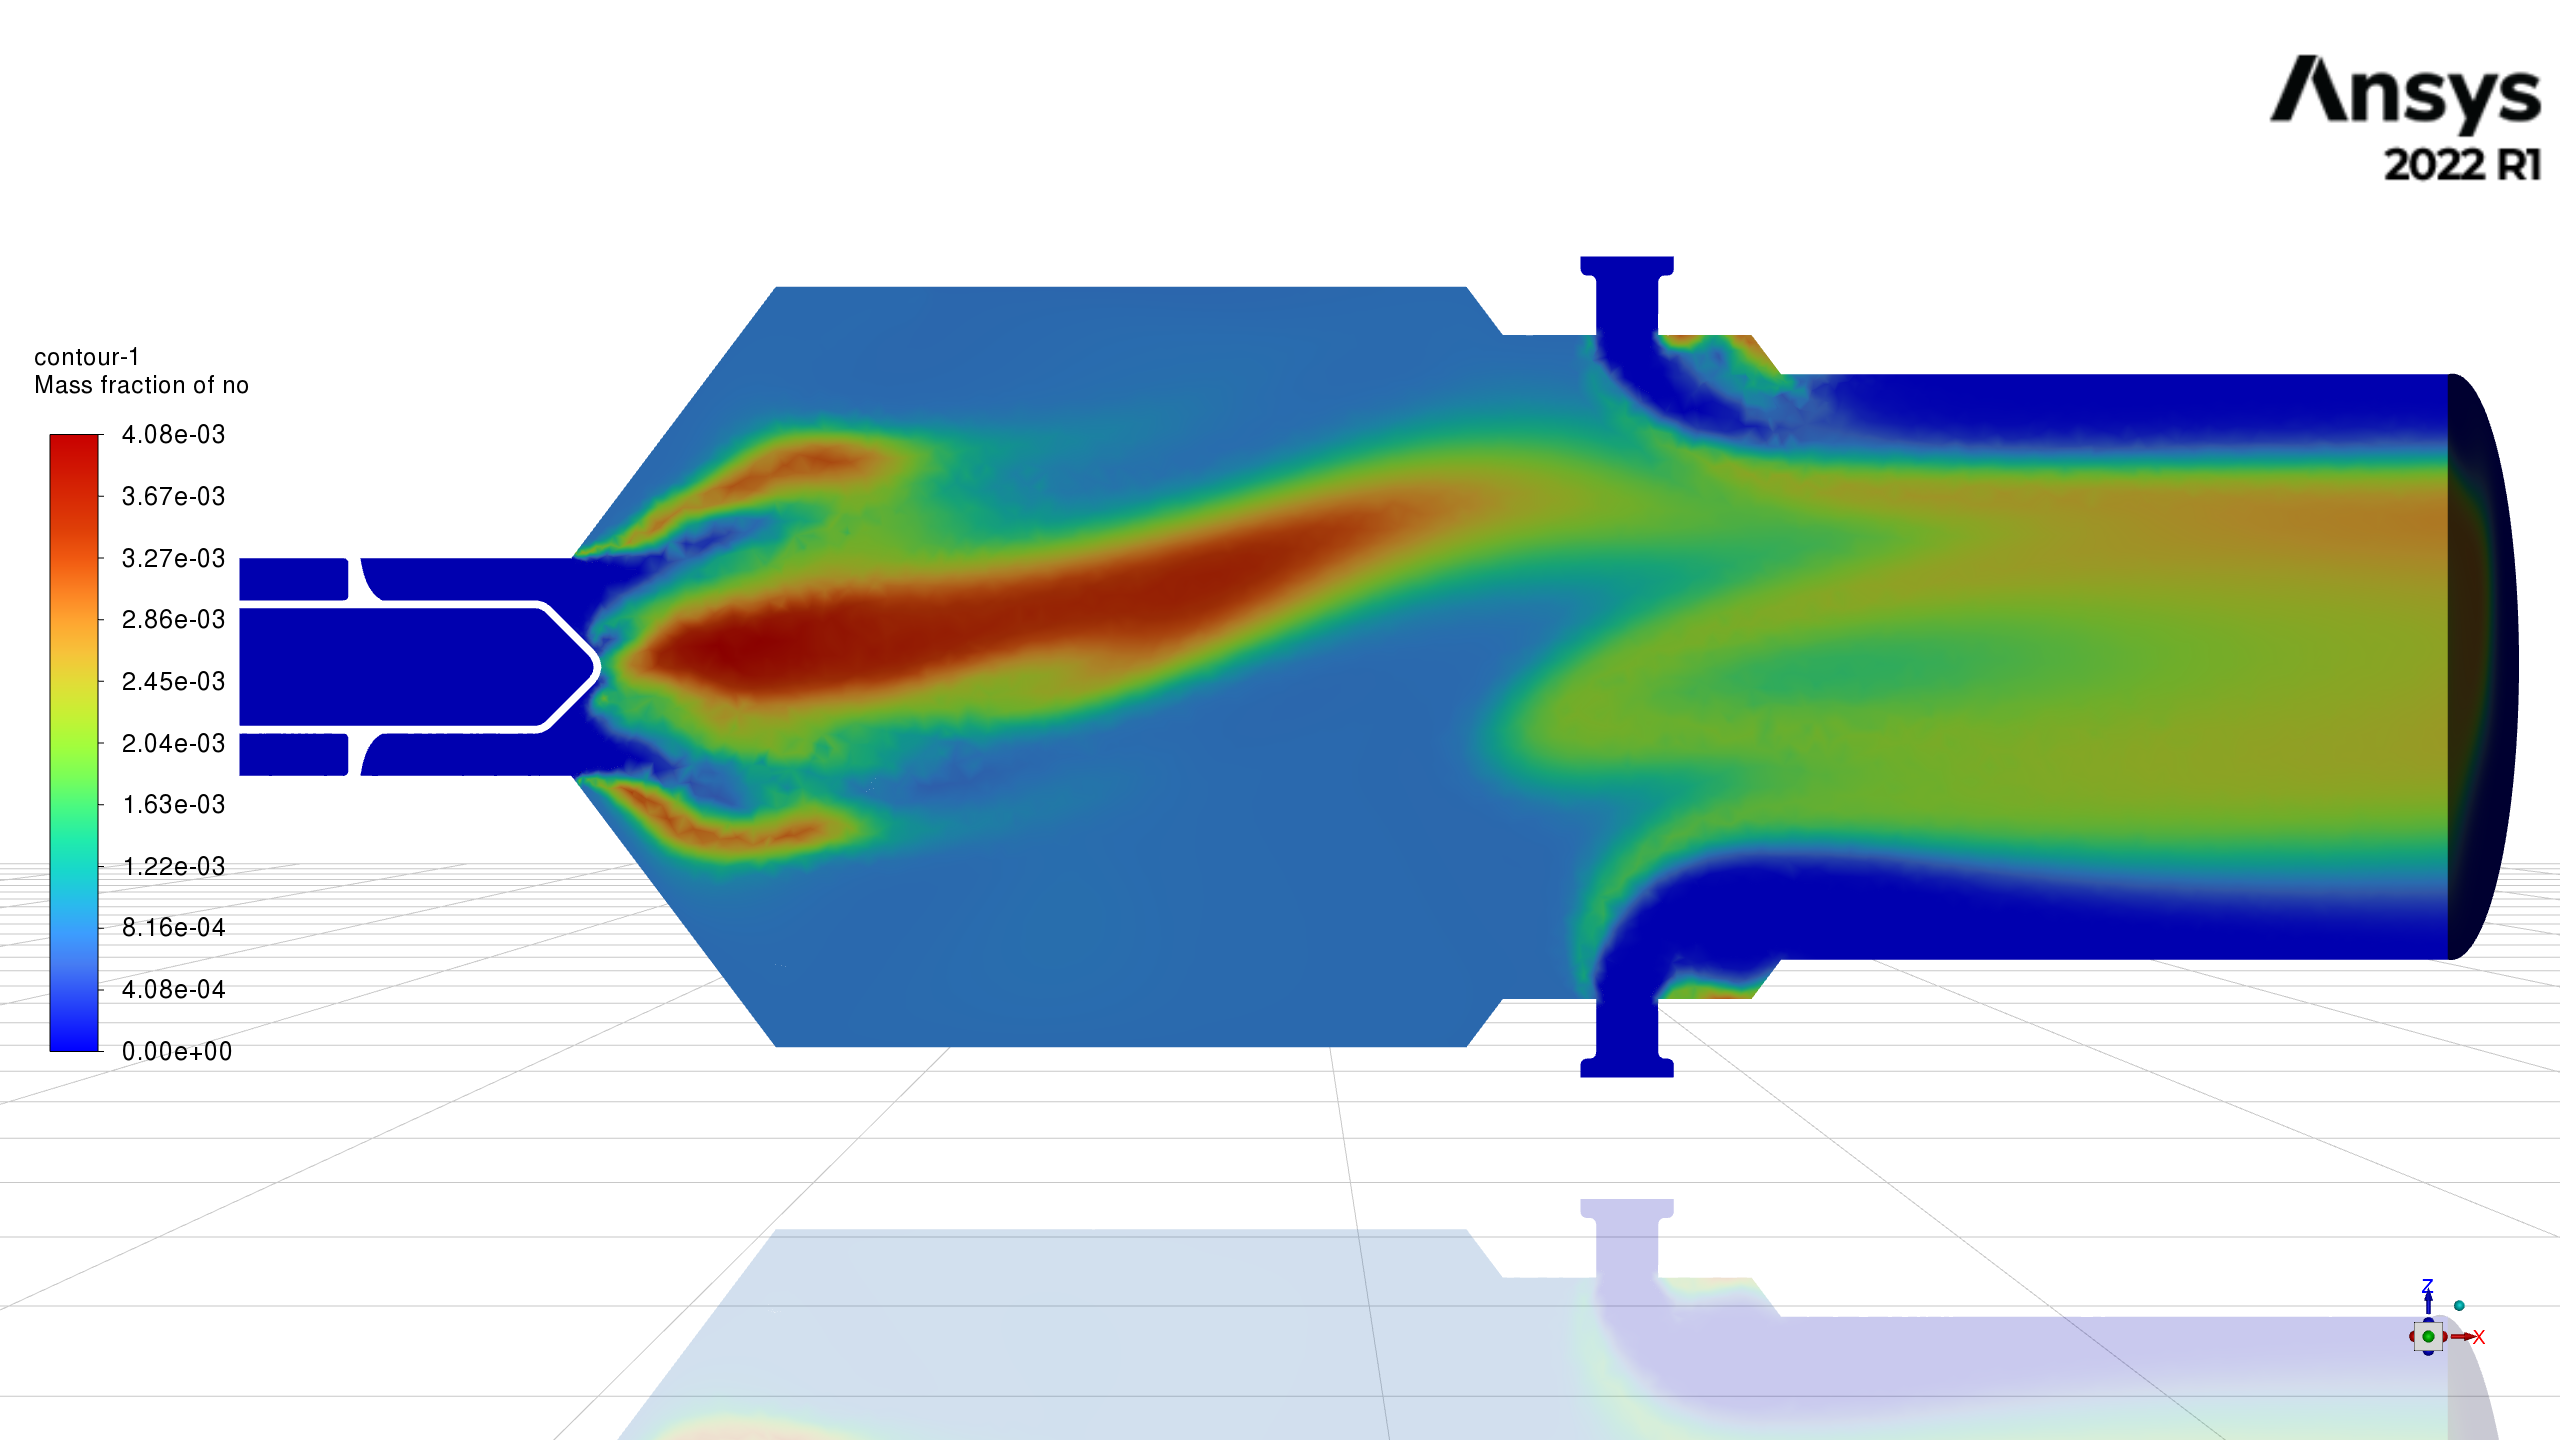
\includegraphics[width=\linewidth]{figs/species_no.png}
        \caption{Species \ce{NO}}\label{fig:nospecies}
    \end{subfigure}

    \caption{Mass fraction of various species across the combustor.}
    \label{fig:species_distro}
\end{figure}


\subsection{Discussion}

\autoref{tab:temp_comp} summarizes the temperatures obtained from cantera analysis as well as numerical analysis using ansys \footnote{Ansys results have been presented by visually looking at the contours presented in the previous subsection}. It can be seen that the temperatures obtained using ansys are higher than the ones computed using cantera. This can probably be due better modelling ability that comes with a 3D numerical simulation instead of simulating flames in 1D.

\begin{table}[H]
    \caption{Temperature comparison.}\label{tab:temp_comp}
    \label{tab:temp_comp}
    \centering
    \begin{tabular}{lll}
    \toprule
    \textbf{Zone} & \textbf{Cantera} & \textbf{ANSYS} \\ 
    \midrule
        Rich Zone & 2217.4 K &   2290 K \\
        Lean Zone & 1675.5 K &   1890 K \\
    \bottomrule
\end{tabular}
\end{table}

When looking at the emission results in \autoref{tab:nox_comp}, the results obtained by cantera are close to what has been seen in the literature in terms of \ce{NOx} production \cite{samuelsen2006rich}. However, the results from ansys show \ce{NOx} results much higher than expected. The reason cannot be determined at the moment.


\begin{table}[H]
    \caption{\ce{NOx} comparison.}\label{tab:nox_comp}
    \label{tab:temp_comp}
    \centering
    \begin{tabular}{lll}
    \toprule
    \textbf{Zone} & \textbf{Cantera} & \textbf{ANSYS} \\ 
    \midrule
    Combustor exit & 58.47 ppm &   2058 ppm \\
    \bottomrule
    \end{tabular}
\end{table}


\subsubsection{Known Errors}

Some know areas of errors are presented below:

\begin{itemize}
    \item Problems with combustion in the lean combustion zone: When performing the analysis using cantera, it was observed that no combustion was taking place in the lean burn zone even though a plug reactor was modelled in that region. The temperature does not change between the mixing zone and the outlet.
    
    \item Problems in the rich zone: At the exit of the rich zone, when looking the mass fraction of all the species, \ce{NH3} was being totally consumed even though the primary zone is supposed to have an equivalence ratio greate that 1. The cause of this problem is unknown and could be the cause of the problem discussed in the previous point.

    \item Limited CFD resources: CFD of reacting flow is time consuming. Therefore, the number of iterations that could be performed for testing and producing the results were limited. There results presented in this report were ran to 500 iterations only. Additionally, no mesh convergence study could be performed due to the same reason. This could have led to the false \ce{NOx} being reported by ansys simulations.
\end{itemize}

\section{Conclusion}
This report shows the effectiveness of RQL combustion in reducing \ce{NOx} emissions from ammonia-fueled systems. The emmision of \ce{NOx} is reduced by using a 3 phase reactor. The first phase is burning ammonia in a fuel-rich environment, then adding secondary air, and finally completing the combustion in a lean zone. The use of Cantera and Ansys validates the results. Cantera showed a significant drop in \ce{NOx} from the rich zone to the lean zone exiting with 55.47 ppm, while ansys simulations show higher outlet levels of \ce{NOx} (2058 ppm), confirming the general trend and highlighting the role of temperature and air mixing in the control of emission. These findings indicate that RQL combustion is a viable approach for enabling cleaner and more controlled ammonia combustion in low-emission gas turbine applications.

\clearpage


\bibliography{sections/mybibfile.bib}


\clearpage

\section*{Appendix A - Function for Primary Section}\label{subsection:primary_calcs}

\begin{minted}[frame=lines,fontsize=\footnotesize,linenos, baselinestretch=1.0]{python}

def primary(save_flag:bool):

    DENSITY_AIR, DENSITY_FUEL, MW_AIR, MW_FUEL = thermo.calc_AirProperties()
    AFR_STOIC = thermo.calc_AirFuelRatio(MW_AIR, MW_FUEL, stoic=True)

    # Design variables
    iters = 51
    V_FUEL_RANGE    =   np.linspace(60, 110, iters)
    V_AIR_RANGE     =   np.linspace(40, 90, iters)

    data_store = []

    for V_FUEL, V_AIR in itertools.product(V_FUEL_RANGE, V_AIR_RANGE):

        mf_fuel         =   DENSITY_FUEL * A_FUEL * V_FUEL
        mf_air_primary  =   DENSITY_AIR  * A_AIR  * V_AIR

        afr_rich        =   mf_air_primary / mf_fuel
        eqr_rich        =   AFR_STOIC / afr_rich

        # Calculate the momentum flux
        momentum_flux = (DENSITY_FUEL * (V_FUEL)**2) / (DENSITY_AIR * V_AIR ** 2)

        data_store.append({
            'EQR_RICH'          :       eqr_rich,
            'AFR_RICH'          :       afr_rich,
            'V_FUEL'            :       V_FUEL,
            'MASSFLOW_FUEL'     :       mf_fuel,
            'V_AIR'             :       V_AIR,
            'MASSFLOW_AIR_P'    :       mf_air_primary,
            'J'                 :       momentum_flux,
        })

    df = pd.DataFrame(data_store)
    print(df)

    df = df[(df['EQR_RICH'] >= 1.24) & (df['EQR_RICH'] < 1.25)]
    df = df[(df['J'] > 2) & (df['J'] < 3)]


    print(df)

    if save_flag:
        df_out = df.round(6)
        ut.make_dir(DATA_DIR)
        df_out.to_csv(os.path.join(DATA_DIR, 'd_points.csv'), index=False)

    if '--plot' in sys.argv:
        
        g = sns.relplot(
            data=df,
            x="EQR_RICH", y="J", col="V_FUEL", hue="V_AIR",
            kind="scatter", palette=palette, col_wrap=3,
            height=4, aspect=.75, facet_kws=dict(sharex=False),
        )

        ut.make_dir(FIG_DIR)

        plt.savefig(FIG_DIR + '/plt_comp.png', format='png')
        plt.savefig(FIG_DIR + '/plt_comp.eps', format='eps')
    
    return AFR_STOIC
\end{minted}

\clearpage

\section*{Appendix B - Function for Secondary Section}

\begin{minted}[frame=lines,fontsize=\footnotesize,linenos, baselinestretch=1.0]{python}
def secondary(silent:bool=True) -> float:

    """
    For the secondary part, the target is to have an equivalence ratio of 0.42.
    How do we get that? Interesting.
    
    """

    DENSITY_AIR, DENSITY_FUEL, MW_AIR, MW_FUEL = thermo.calc_AirProperties()
    AFR_STOIC = thermo.calc_AirFuelRatio(MW_AIR, MW_FUEL, stoic=True)

    # Following is the desgin point selected from the primary calculations.
    EQR_GLOBAL:float = 0.42
    PRIMARY_VARS:dict = {
        'EQR_RICH': 1.245,
        'AFR_RICH': 4.854891, 
        'V_FUEL': 99.0, 
        'MASSFLOW_FUEL': 0.007339, 
        'V_AIR': 65.0, 
        'MASSFLOW_AIR_P': 0.035631, 
        'J': 2.738813
        }

    MASSFLOW_AIR_P = PRIMARY_VARS['MASSFLOW_AIR_P']
    AFR_GLOBAL = AFR_STOIC / EQR_GLOBAL
    MASSFLOW_AIR_GLOBAL = PRIMARY_VARS['MASSFLOW_FUEL'] * AFR_GLOBAL

    MASSFLOW_AIR_S = MASSFLOW_AIR_GLOBAL - MASSFLOW_AIR_P

    if silent:
        print(MASSFLOW_AIR_S)
        return MASSFLOW_AIR_S
    else:
        print("")
        print('Combustor mass flows:')
        print(f"{'Quantity':<20} {'Value':>15} {'Unit':<10}")
        print("-" * 50)
        print(f"{'Global mass flow':<20} {MASSFLOW_AIR_GLOBAL:>15.6f} {'kg/m3':<10}")
        print(f"{'Primary mass flow':<20} {PRIMARY_VARS['MASSFLOW_AIR_P']:>15.6f} {'kg/m3':<10}")
        print(f"{'Secondary mass flow':<20} {MASSFLOW_AIR_S:>15.6f} {'kg/m3':<10}")

\end{minted}

\clearpage


\section*{Appendix B - Functions for RQL reactor in Cantera}


\textbf{RICH ZONE}

\begin{minted}[frame=lines,fontsize=\footnotesize,linenos, baselinestretch=1.0]{python}
def rich(
    eqr: float, mixture:ct.composite.Solution
) -> tuple:
    """
    Function for calculating the reaction characteristics in the rich burn zone.
   
    Inputs:
    ------
    - eqr_rich: equivalence ratio for the rich zone
    - air: cantera air
    - fuel: cantera fuel
    - mixture: init mixture gas
   
    Returns:
    -------
    - flame: solved FreeFlame object
    - gas_mix: cantera Solution object with the mixed state
    - outlet_state: string of species mass fractions at the outlet
    """

    # Solve flame simulation
    initial_grid = np.linspace(0, 0.059917, 101)
    flame = ct.FreeFlame(mixture, initial_grid)
    flame.energy_enabled = True
    flame.set_refine_criteria(ratio=3, slope=0.2, curve=0.2)
    
    try:
        flame.solve(loglevel=1, refine_grid=True, auto=False)
        solution_successful = True
    except:
        flame.set_refine_criteria(ratio=3, slope=0.1, curve=0.1)
        try:
            flame.solve(loglevel=1, refine_grid=True, auto=True)
            solution_successful = True
        except:
            solution_successful = False
    
    if solution_successful:
        print(f'Phi={eqr}: Outlet temperature = {flame.T[-1]:.1f} K')
        try:
            no_index = mixture.species_index('NO')
            print(f'NOx at outlet: {1000000*flame.Y[no_index][-1]:.2f} ppm')
        except ValueError:
            print("NO species not found in mechanism")

        outlet_state = ''
        #print("\n\n")
        #print(f"{'Species':<20} {'Mass Fraction':>15}")
        #print("-" * 50)
        for i in range(0, mixture.n_species):
            species_name = mixture.species_name(i)
            species_mass_fraction = flame.Y[mixture.species_index(species_name)][-1]
            if i == 0:
                outlet_state += f'{species_name}:{species_mass_fraction:.9f}'
            else:
                outlet_state += f',{species_name}:{species_mass_fraction:.9f}'
            #print(f"{species_name:<20} {species_mass_fraction:>15.9f}")
        #print("\n\n")

        return flame, mixture, outlet_state
    
    else:
        print("Flame solution failed. Returning None.")
        return None, mixture, None

\end{minted}

\clearpage


\textbf{MIXING ZONE}

\begin{minted}[frame=lines,fontsize=\footnotesize,linenos, baselinestretch=1.0]{python}
def mixing(
    gas_a:ct.composite.Solution, gas_b:ct.composite.Solution, mdot_a:float, mdot_b:float
) -> tuple:
    """
    Description:
    -----------
    This function mixes two gases.
    https://cantera.org/3.1/examples/python/reactors/mix1.html#sphx-glr-examples-python-reactors-mix1-py

    Inputs:
    ------
    gas_a: This is the combustion gas obtained from the first part of the reaction.
    gas_b: This is the quench air obtained from the HPC.
    EQR  : The equivalence ratio of the mixture.

    Returns:
    ------
    boundary species for lean burn
    
    """

    # Create reservoirs for storing mixture data.
    reservoir_a = ct.Reservoir(gas_a, name='gas a res')
    reservoir_b = ct.Reservoir(gas_b, name='gas b res')
    downstream  = ct.Reservoir(gas_b, name='outlet reservoir')

    # Create a reactor for the mixer. A reactor is required instead of a reservoir, 
    # since the state will change with time if the inlet mass flow rates change or if there 
    # is chemistry occurring. FROM CANTERA DOCUMENTATION
    mixer = ct.IdealGasReactor(gas_a, name='Mixer')

    # Create the mass flow controllers.
    mfc1 = ct.MassFlowController(reservoir_a, mixer, mdot=mdot_a, name="gas_a")
    mfc2 = ct.MassFlowController(reservoir_b, mixer, mdot=mdot_b, name="gas_b")


    outlet = ct.Valve(mixer, downstream, K=10.0, name="Valve")
    sim = ct.ReactorNet([mixer])

    sim.advance_to_steady_state()
    print(mixer.thermo.report())

    # Prepare the species from this reactor to the one with Lean burner calculation
    boundary_species:str = ''
    for i in range(100000):
        try:
            name = mixer.thermo.species_name(i)
            y_val = mixer.thermo.Y[mixer.thermo.species_index(name)]
            if i == 0:
                boundary_species += '%s:%.8f'%(name,y_val)
            else:
                boundary_species += ' ,%s:%.8f'%(name,y_val)
        except:
            break
   
    return mixer, boundary_species
\end{minted}

\clearpage

\textbf{LEAN ZONE}

\begin{minted}[frame=lines,fontsize=\footnotesize,linenos, baselinestretch=1.0]{python}
def lean(
    gas:ct.composite.Solution, mdot:float, geom:dict
) -> None:
    print("Computing LEAN zone.")

    n_steps = 2000
    dz = geom['length'] / n_steps
    r_vol = geom['area'] * dz

    # Make a new reactor for lean burn
    lean_reactor = ct.IdealGasReactor(gas)
    lean_reactor.volume = r_vol
    upstream = ct.Reservoir(gas, name='upstream')
    downstream = ct.Reservoir(gas, name='downstream')
    m = ct.MassFlowController(upstream, lean_reactor, mdot=mdot)
    v = ct.PressureController(lean_reactor, downstream, primary=m, K=1e-5)
    sim2 = ct.ReactorNet([lean_reactor])

    # define time, space, and other information vectors
    z2 = (np.arange(n_steps) + 1) * dz
    t_r2 = np.zeros_like(z2)  # residence time in each reactor
    u2 = np.zeros_like(z2)
    t2 = np.zeros_like(z2)
    states2 = ct.SolutionArray(lean_reactor.thermo)

    # iterate through the PFR cells
    for n in range(n_steps):
        # Set the state of the reservoir to match that of the previous reactor
        gas.TDY = lean_reactor.thermo.TDY
        upstream.syncState()
        # integrate the reactor forward in time until steady state is reached
        sim2.reinitialize()
        sim2.advance_to_steady_state()
        # compute velocity and transform into time
        u2[n] = mdot / geom['area'] / lean_reactor.thermo.density
        t_r2[n] = lean_reactor.mass / mdot  # residence time in this reactor
        t2[n] = sum(t_r2)
        # write output data
        states2.append(lean_reactor.thermo.state)

    print('Final Temperature is ',states2.T,'K')
    print(f"NOx is {1000000*states2.Y[-1, gas.species_index('NO')]} ppm")

    return gas
\end{minted}


\clearpage


\textbf{RQL Function}

\begin{minted}[frame=lines,fontsize=\footnotesize,linenos, baselinestretch=1.0]{python}
def RQL(
    eqr_rich:float, eqr_lean:float
) -> None:
    """
    NOTE:
    This function should have 3 parts:
    1. Rich burn reaction.
    2. Mixing of the secondary air.
    3. Lean burn reaction.

    And also two misc steps:
    1. Before the program runs, need to generate directories.
    """
    print("Initializing the RQL reaction mechanism.")

    # TODO Perform the preprocessing step:
    # Create temp directories for storing data between separate RQL stages.
    # INIT gases

    PFR:dict = {
        'length': 0.5,     # [m]
        'radius': 0.018823,     # [m]
        'area'  : 1.e-3,     # [m^2]
        'volume': 0.000048,     # [m^3]
        'vel'   : 20            # [m/s] 
    }

    fuel        = ct.Solution(SanDiegoMech)
    fuel.TPX    = T_FUEL, P_FUEL, {'NH3': 1.0}

    air         = ct.Solution(SanDiegoMech)
    air.TPX     = T_AIR, P_AIR, {'O2': 1.0, 'N2': 3.76}

    rich_gas_thermo, inlet_bounbdary_species = rt.mixing(gas_a=fuel, gas_b=air, mdot_a=0.007339, mdot_b=0.035631)
    
    # Create the rich burn gas
    rich_gas = ct.Solution(SanDiegoMech)    
    rich_gas.TPY = rich_gas_thermo.thermo.T, rich_gas_thermo.thermo.P, rich_gas_thermo.thermo.Y
    rich_flame, rich_out, rich_outlet_state = rt.rich(eqr=1.24, mixture=rich_gas)
    print(rich_out.report())

    air_secondary         = ct.Solution(SanDiegoMech)
    air_secondary.TPX     = T_AIR, P_AIR, {'O2': 3.0, 'N2': 3*3.76}

    # Mix the output of rich flame with secondary air.
    lean_gas_thermo, lean_inlet_boundary_species = rt.mixing(gas_a=rich_out, gas_b=air_secondary, mdot_a=0.007339+0.035631, mdot_b=secondary())
    
    # Create the lean burn gas
    lean_gas = ct.Solution(SanDiegoMech)
    lean_gas.TPY = lean_gas_thermo.thermo.T, lean_gas_thermo.thermo.P, lean_gas_thermo.thermo.Y
    print(lean_gas.report())
\end{minted}

\clearpage

\section*{Appendix D - RQL Combustor Drawing} \label{subsection:rql_dim_drawing}


\begin{figure}[H]
    \centering
    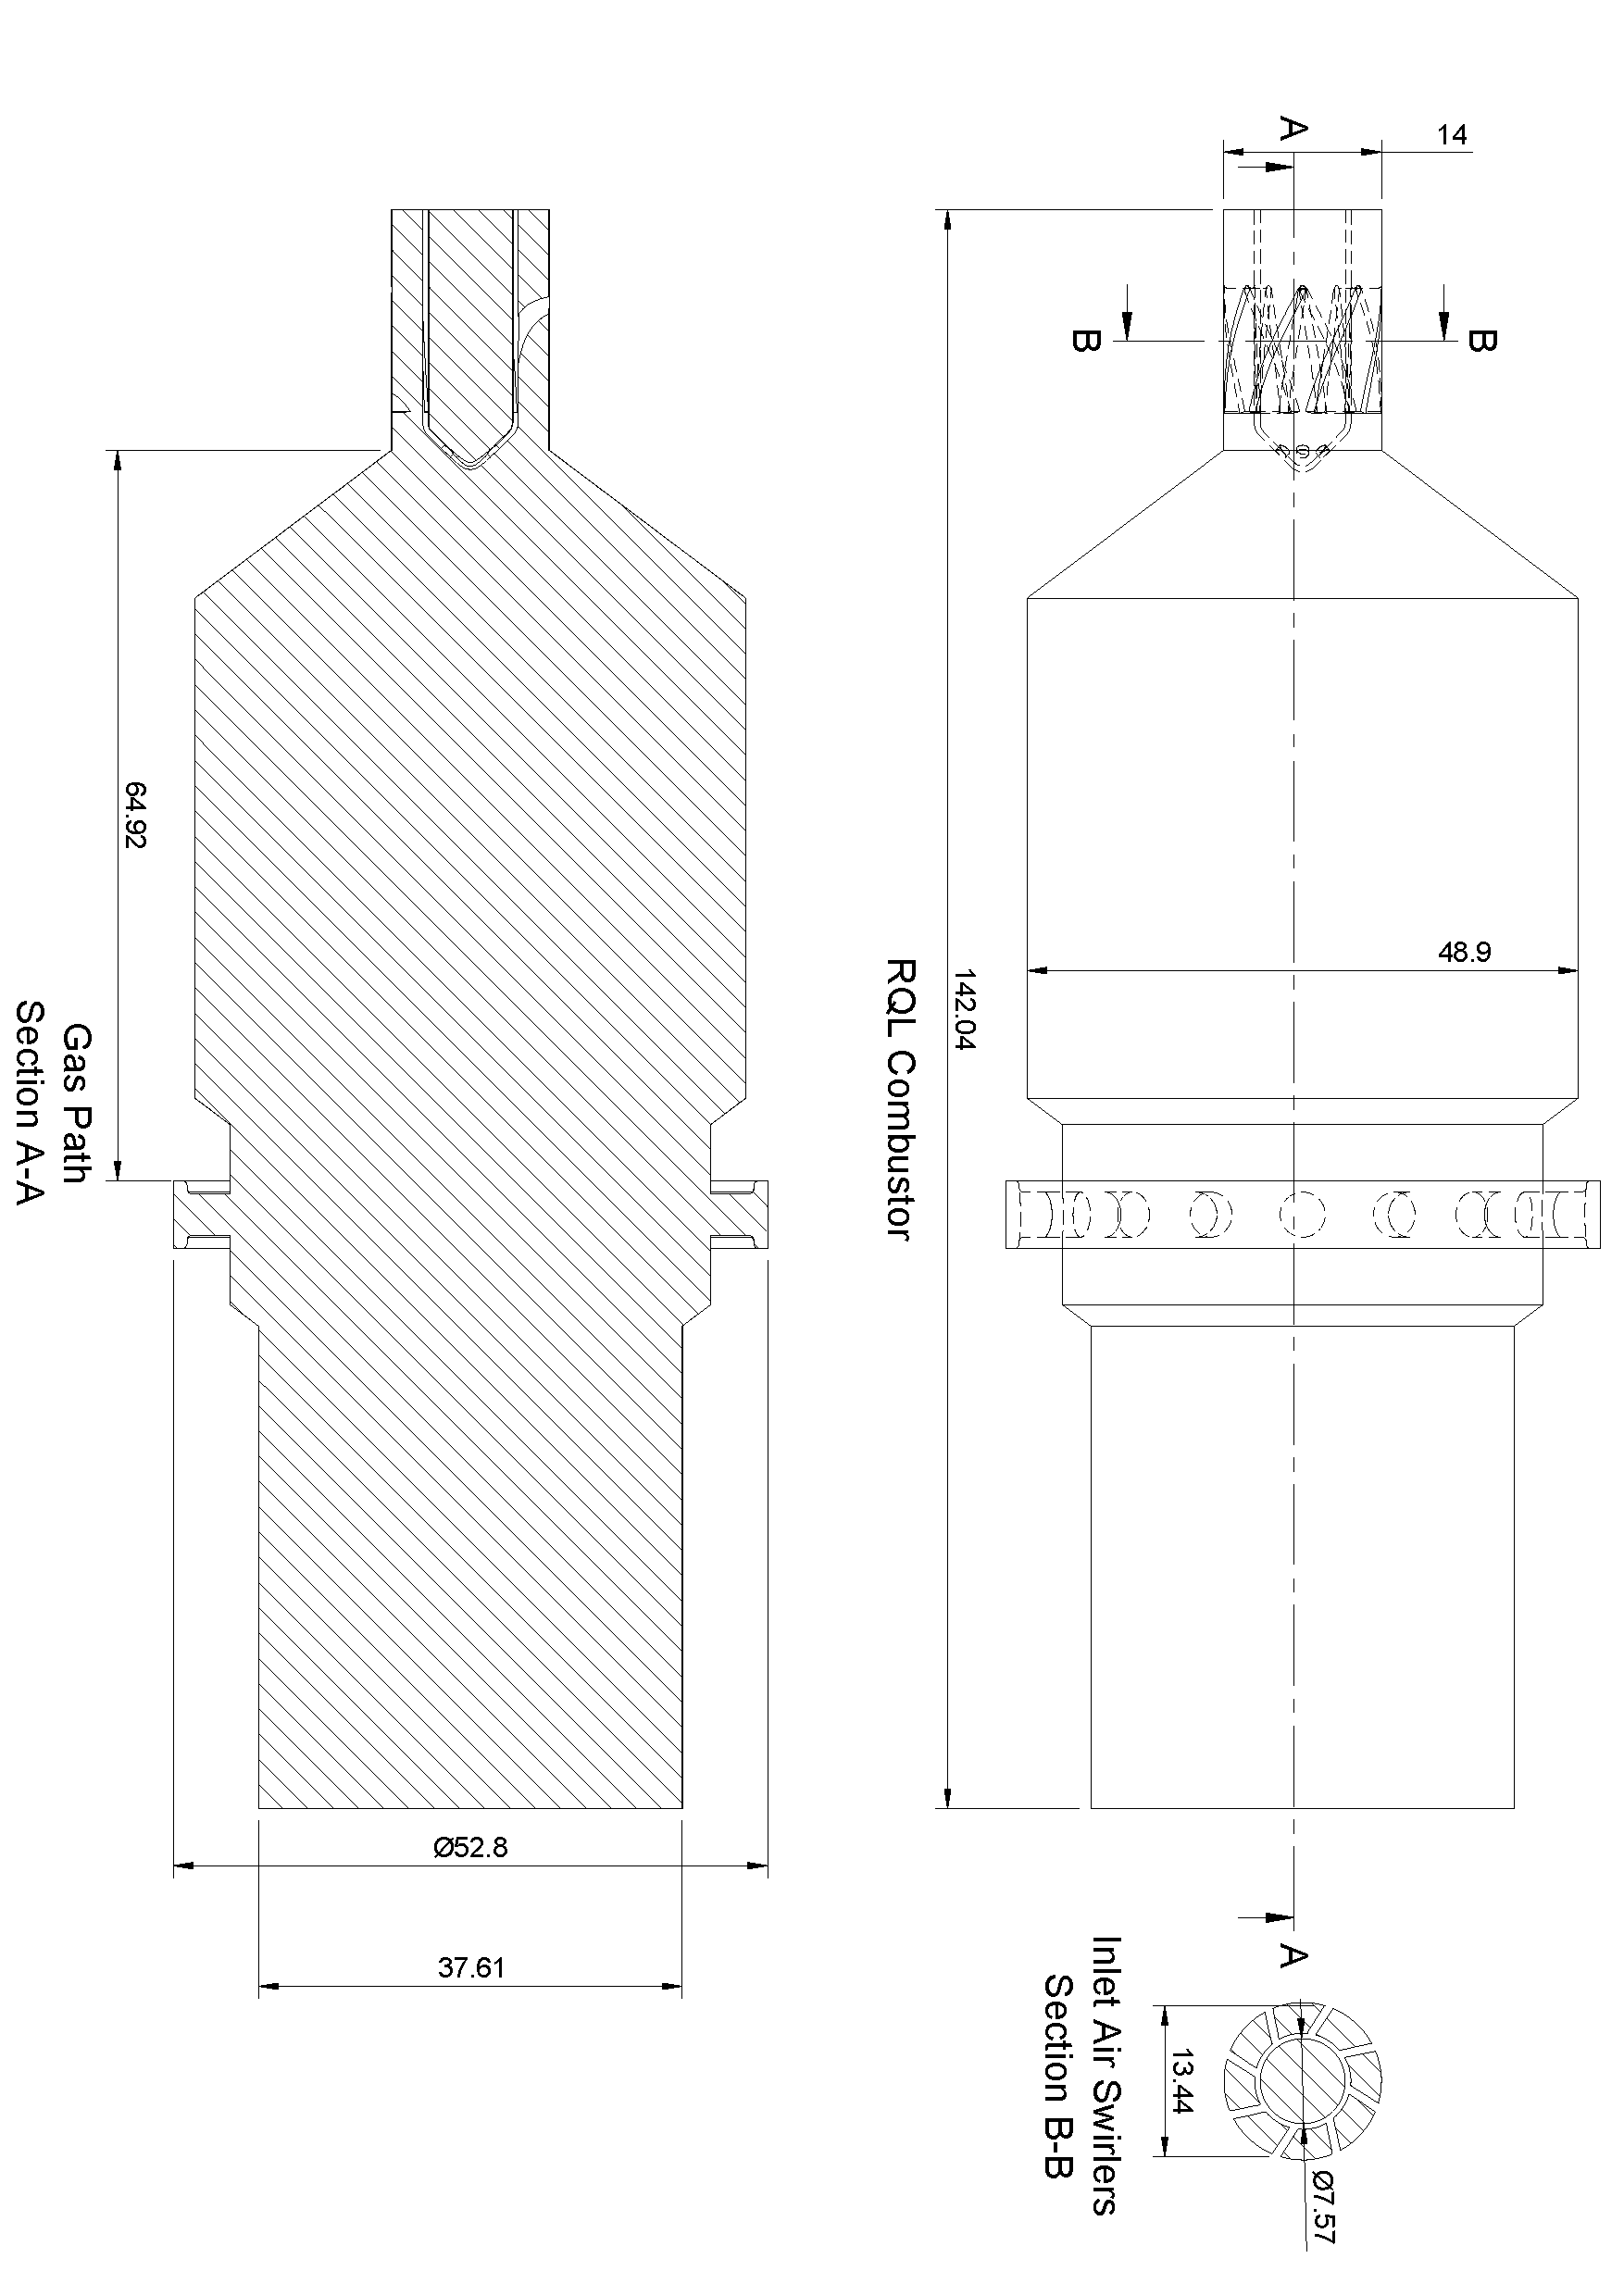
\includegraphics[width=0.9\linewidth]{figs/RQL Combustor DWG.pdf}
    \caption{Drawing for the RQL combustor.}
    \label{fig:Drawing_RQL}
\end{figure}

\end{document}